\documentclass[a4paper,10pt]{article}

\usepackage[hidelinks]{hyperref}
\usepackage{float}
\usepackage{amsmath}
\usepackage{fixltx2e} % (vecchio)

% Lingua
\usepackage[utf8]{inputenc}
\usepackage[italian]{babel}

% Margini
\usepackage{geometry}
\geometry{a4paper, top=3cm, bottom=3cm, left=3cm, right=3cm}
\setlength{\parindent}{0pt}

\usepackage{graphicx}   % per immagini
\usepackage{hyperref}   % per link
\usepackage{caption}    % per didascalie
\captionsetup[table]{labelformat=empty}
\usepackage{ifthen}     % per \ifthenelse
\usepackage{longtable}

\usepackage{tikz}

\usepackage{array}      % per tabelle
\newcolumntype{M}[1]{>{\centering\arraybackslash}m{#1}}

\usepackage{datetime}

% Definisci un formato personalizzato
\newdateformat{italianformat}{\THEDAY~\monthname[\THEMONTH]~\THEYEAR}
\newdate{dataverbale}{12}{01}{2026}

% Definizione del formato con le barre
\newdateformat{slashdate}{\twodigit{\THEDAY}/\twodigit{\THEMONTH}/\THEYEAR}

% Per logo in ogni pagina
\usepackage{eso-pic}
\usepackage{tikz}
\AddToShipoutPictureBG{%
  \ifthenelse{\value{page}>1}{%
    \begin{tikzpicture}[remember picture, overlay]
      % Icona
      \node[anchor=north west, inner sep=0pt] at ([xshift=28pt,yshift=-28pt]current page.north west) 
        {
\includegraphics[width=1cm, height=1cm]{resources/Tool-8_icon_white.png}};
      
      % Riga
      \draw[black, line width=0.5pt] ([xshift=28pt + 1cm, yshift=-28pt - 0.6cm]current page.north west) 
            -- ++(3cm, 0);
      % Testo
      \node[anchor=west, text=black, font=\small] at ([xshift=28pt + 1cm, yshift=-28pt - 0.4cm]current page.north west) 
        {Piano di Qualifica};
    \end{tikzpicture}
  }{}
}


%------Ridefinizione maketitle-------
\makeatletter
\renewcommand{\maketitle}{%
  \vspace*{\fill}
  \begin{center}
    {\LARGE \bfseries \@title \par}
    \vskip 1em
    {\large \@author \par}
    \vskip 1em
    {\large\slashdate{\displaydate{dataverbale}} \par}
  \end{center}
  \vspace*{\fill}
}
\makeatother
%-----------------------------------

\title{%
  
\includegraphics[width=10cm]{resources/Tool-8_white_2.png} \\[1.5ex]
  \textbf{\LARGE Piano di Qualifica}
}
\author{}
\date{\dataverbale}
\begin{document}
\tikz[remember picture,overlay] \node[opacity=0.2,inner sep=0pt] at (current page.center){
\includegraphics[width=\paperwidth,height=\paperheight]{resources/Abstract_lines.png}};

\maketitle

\newpage

\section*{Revisioni}
\begin{table}[h!]
\centering
\begin{tabular}{|M{0.8cm}|p{3cm}|p{4.1cm}|M{1.8cm}|p{3cm}|}
  \hline
  \textbf{Ver.} & \textbf{Autore} & \textbf{Modifiche} & \textbf{Data} & \textbf{Verifica} \\
  \hline
  1.7 & Besnik Murtezan & Aggiornamento grafici del cruscotto con Sprint 11 e 12 & 09/05/2026 & Stefano Maso \\
  \hline
  1.6 & Stefano Maso & Aggiunte metriche per il processo di verifica, aggiunti test di integrazione, aggiunte sezioni cruscotto & 03/05/2026 & Besnik Murtezan \\
  \hline
  1.5 & Stefano Maso & Aggiornamento grafici del cruscotto con Sprint 10 e aggiunta Test di Unità & 29/04/2026 & Spadiliero Ruben \\
  \hline
  1.4 & Spadiliero Ruben & Aggiornamento grafici del cruscotto con Sprint 9 & 24/04/2026 & Banchieri Giuliano \\
  \hline
  1.3 & Giuliano Banchieri & Aggiornamento grafici del cruscotto con Sprint 8 & 17/04/2026 & Spadiliero Ruben \\
  \hline
  1.2 & Gabriele Disa & Aggiornati grafici del cruscotto con Sprint 7 (insieme all'analisi), aggiornato indice di Gulpease con Manuale Utente e Specifica Tecnica & 13/04/2026 & Besnik Murtezan \\
  \hline
  1.1 & Giuliano Banchieri & Aggiunta test di unità & 09/04/2026 & Besnik Murtezan \\
  \hline
  1.0 & Besnik Murtezan & Approvazione documento per RTB & 25/03/2026 & Stefano Maso \\
  \hline
  0.6 & Niccolò Feltrin & Aggiornati grafici del cruscotto con Sprint 6 (insieme all'analisi) & 25/03/2026 & Stefano Maso \\
  \hline
  0.5 & Niccolò Feltrin & Aggiornati grafici del cruscotto con Sprint 5 (insieme all'analisi), aggiornato indice di Gulpease con verbale esterno 16/03/2026 e interno 18/03/2026 & 24/03/2026 & Stefano Maso \\
  \hline
  0.4 & Niccolò Feltrin & Aggiornato calcolo indice di Gulpease in AdR (v1.0) e verbale interno 3/3/2026, aggiunti test di sistema & 10/03/2026 & Giuliano Banchieri \\
  \hline
  0.3 & Niccolò Feltrin & Aggiornati grafici del cruscotto con Sprint 4 (insieme all'analisi), e aggiunto calcolo dell'indice di Gulpease su verbali e documenti per RTB & 06/03/2026 & Giuliano Banchieri \\
  \hline
  0.2 & Stefano Maso & Aggiornamento Cruscotto di valutazione a seguito del terzo sprint & 17/02/2026 & Besnik Murtezan \\
  \hline
  0.1 & Stefano Maso & Prima stesura documento completo & \slashdate{\displaydate{dataverbale}} & Besnik Murtezan \\
  \hline
\end{tabular}
\label{tab:revisioni}
\end{table}

\newpage

\tableofcontents

\newpage

\section{Introduzione}
\subsection{Scopo del documento}
Il Piano di Qualifica$^G$ definisce le metriche di valutazione del prodotto, sulla base dei requisiti e delle aspettative della proponente$^G$, in modo da poter definire la qualità del prodotto attraverso un processo di continuo miglioramento.
Il Piano di Qualifica$^G$ è concepito per essere incrementale e dinamico, soprattutto per quanto riguarda le metriche descritte e punta a dare una valutazione il più oggettiva possibile di ciò che è stato realizzato. Eventuali termini tecnici sono definiti all'interno del documento "Glossario".
\subsection{Riferimenti}
\subsubsection{Riferimenti normativi}
\begin{itemize}
    \item \href{https://tool-8.github.io/Documentazione-SWE/}{Norme di Progetto v1.0}
    \item Capitolato$^G$ C6 - Progetto$^G$ Second Brain:    \\ \url{https://www.math.unipd.it/~tullio/IS-1/2025/Progetto/C6.pdf}
\end{itemize}
\subsubsection{Riferimenti informativi}
\begin{itemize}
    \item Lezione \textit{Progettazione$^G$ Software (T6)} del corso di \textit{Ingegneria del software$^G$}: \\ \url{https://www.math.unipd.it/~tullio/IS-1/2025/Dispense/T06.pdf}
    \item Lezione \textit{Qualità di prodotto (T7)} del corso di \textit{Ingegneria del software$^G$}: \\ \url{https://www.math.unipd.it/~tullio/IS-1/2025/Dispense/T0.pdf}
    \item Lezione \textit{Qualità di processo (T8)} del corso di \textit{Ingegneria del software$^G$}: \\ \url{https://www.math.unipd.it/~tullio/IS-1/2025/Dispense/T08.pdf}
    \item Lezione \textit{Verifica$^G$ e validazione$^G$: introduzione (T9)} del corso di \textit{Ingegneria del software$^G$}: \\ \url{https://www.math.unipd.it/~tullio/IS-1/2025/Dispense/T09.pdf}
    \item Lezione \textit{Verifica$^G$ e validazione$^G$: analisi statica (T10)} del corso di \textit{Ingegneria del software$^G$}: \\ \url{https://www.math.unipd.it/~tullio/IS-1/2025/Dispense/T10.pdf}
    \item Lezione \textit{Verifica$^G$ e validazione$^G$: analisi dinamica aka testing (T11)} del corso di \textit{Ingegneria del software$^G$}: \\ \url{https://www.math.unipd.it/~tullio/IS-1/2025/Dispense/T11.pdf}
    \item Metriche di progetto$^G$ (\textit{Earned Value Analysis}): \\ \url{https://it.wikipedia.org/wiki/Metriche_di_progetto}
\end{itemize}
\subsection{Codifica delle metriche}
Una metrica è identificata dal seguente formato di codice: 
\begin{center}
    [Tipo][Id]-[Acronimo]
\end{center}
\begin{itemize}
    \item \textbf{Tipo}: può essere PC (per un processo) o PD (per un prodotto)
    \item \textbf{Id}: identificativo all'interno di un certo tipo di metrica
    \item \textbf{Acronimo}: acronimo del nome della metrica
\end{itemize}
Ogni metrica avrà una descrizione, i valori accettabili e quelli preferibili.

\section{Qualità di processo}
La qualità è determinata dai processi che la compongono, misurata scegliendo delle buone metriche di misurazione di qualità e anche buoni strumenti (serve automazione e oggettività). 
\subsection{Processi primari}
\subsubsection{Fornitura}
Per definire le metriche adottate per i processi primari di fornitura andremo a fare riferimento alla tecnica denominata \textit{EVA} (\textit{Earned Value Analysis}) che consenste di calcolare in termini di tempo, denaro speso e valore del lavoro realizzato e di valutare le performance del progetto.\\ Tra queste individuiamo:
\begin{itemize}
    \item \textbf{Budget at Completion (BAC)}: valore previsto inizialmente per la realizzazione del progetto$^G$
    \item \textbf{Estimated at Completion (EAC)}: revisione del valore stimato per la realizzazione del progetto$^G$
    \item \textbf{Planned Value (PV)}: costo previsto per realizzare le attività di progetto$^G$ per la data stabilita (tempo o denaro)
    \item \textbf{Actual Cost (AC)}: costo effettivamente sostenuto alla data stabilita (tempo o denaro)
    \item \textbf{Earned Value (EV)}: valore delle attività sostenute alla data stabilita (tempo o denaro)
    \item \textbf{Estimated to Complete (ETC)}: valore stimato per completare le attività rimanenti necessarie per concludere il progetto$^G$
    \item \textbf{Cost Variance (CV)}: misura la variazione del valore ottenuto (EV) rispetto al costo effettivo (AC)
    \item \textbf{Schedule Variance (SV)}: misura la variazione del valore ottenuto (EV) rispetto al costo pianificato (PV)
    \item \textbf{Budget Variance (BV)}: misura la variazione dal costo attuale (AC) rispetto al costo atteso (CV)
\end{itemize}
Come riportato dal documento Dichiarazione di Impegni, il BAC corrisponde ad un valore di \textbf{€ 10.950,00}.
\\
Obiettivi di qualità per tali metriche: 
\begin{table}[H]
\centering
\renewcommand{\arraystretch}{1.2}
\begin{tabular}{|l|l|c|c|}
\hline
\textbf{Metrica} & \textbf{Nome} & \textbf{Valore Accettabile} & \textbf{Valore Preferibile} \\
\hline
PC01-EAC & Estimated at Completion & $\pm 5\%$ BAC & = BAC \\
PC02-PV  & Planned Value           & $\geq 0$      & $\leq$ BAC \\
PC03-AC  & Actual Cost             & $\geq 0$      & $\leq$ EAC \\
PC04-EV  & Earned Value             & $\geq 0$      & $\leq$ EAC \\
PC05-ETC & Estimated to Complete    & $\geq 0$      & $\leq$ EAC \\
PC06-CV  & Cost Variance            & $\geq -7.5\%$ & $\geq 0$ \\
PC07-SV  & Schedule Variance        & $\geq -7.5\%$ & $\geq 0$ \\
PC08-BV  & Budget Variance          & $\pm 10\%$    & = 0 \\
\hline
\end{tabular}
\caption{Metriche per i processi di fornitura}
\label{tab:metriche-fornitura}
\end{table}
\subsubsection{Sviluppo}
\textbf{Analisi dei Requisiti} Per l'attività di \textit{Analisi dei Requisiti$^G$} definiamo le seguenti metriche:
\begin{itemize}
    \item \textbf{Requirements stability index (RSI)}: misura la stabilità dei requisiti nel corso del tempo durante lo sviluppo$^G$ del progetto$^G$; è misurata nel suguente modo:
    \begin{center}
        \[
        RSI = 1 - \left( \frac{N_{\text{modifiche}}}{N_{\text{requisiti totali}}} \right) \times 100
        \]
    \end{center}
    Dove: \\
    - N\textsubscript{modifiche} è il numero totale di modifiche apportate ai requisiti durante un periodo di tempo specifico \\
    - N\textsubscript{requisiti totali} è il numero totale di requisiti del progetto$^G$
\end{itemize}
\textbf{Progettazione} Per l'attività di progettazione$^G$ definiamo le seguenti metriche:
\begin{itemize}
    \item \textbf{Structural fan-in (SFIN)}: misura la quantità dei moduli che utilizzano un modulo specifico, un valore alto significa che molte parti del sistema dipendono da un modulo in particolare
    \item \textbf{Structural fan-out (SFOUT)}: misura il numero di moduli utilizzati da un modulo specifico, un valore alto significa che il modulo considerato dipende da molti altri moduli
\end{itemize}
\textbf{Codifica} Per l'attività di codifica definiamo le seguenti metriche:
\begin{itemize}
    \item \textbf{Linee di codice (LOC)}: misura la complessità del software in base al numero di linee di codice sorgente
\end{itemize}
Obiettivi per tali metriche:
\begin{table}[H]
\centering
\renewcommand{\arraystretch}{1.2}
\begin{tabular}{|l|l|c|c|}
\hline
\textbf{Metrica} & \textbf{Nome} & \textbf{Valore Accettabile} & \textbf{Valore Preferibile} \\
\hline
PC09-RSI & Requirements stability index & $\geq 70\%$ & $100\%$ \\
PC10-SFIN  & Structural fan-in           & -      & Masismo \\
PC11-SFOUT  & Structural fan-out            & -      & Minimo \\
PC12-LOC  & Linee di codice             & $\leq 50.000$      & $\leq 30.000$  \\
\hline
\end{tabular}
\caption{Metriche per i processi di sviluppo}
\label{tab:metriche-sviluppo}
\end{table}

\subsection{Processi di supporto}
\subsubsection{Documentazione} 
Per il processo di documentazione definiamo le seguenti metriche:
\begin{itemize}
    \item \textbf{Errori ortografici (EO)}: misura la quantità di errori ortografici individuati per documento
    \item \textbf{Indice Gulpease (IG)}: misura la leggibilità di un documento in lingua italiana, calcolato nel seguente modo:
        \[
        IG = 89 + \frac{300 \times (num. frasi) - 10 \times (num. lettere) }{num. parole}
        \]
    Dove: \\
    - \textit{num. frasi} è il numero di frasi nel documento \\
    - \textit{num. lettere} è il numero di lettere nel documento \\
    - \textit{num. parole} è il numero di parole nel documento
\end{itemize}
Obiettivi per tali metriche:
\begin{table}[H]
\centering
\renewcommand{\arraystretch}{1.2}
\begin{tabular}{|l|l|c|c|}
\hline
\textbf{Metrica} & \textbf{Nome} & \textbf{Valore Accettabile} & \textbf{Valore Preferibile} \\
\hline
PC13-EO & Errori ortografici & 0 & 0 \\
PC14-IG  & Indice Gulpease & 40-100      & 55-100 \\
\hline
\end{tabular}
\caption{Metriche per i processi di supporto}
\label{tab:metriche-supporto}
\end{table}
\subsubsection{Verifica}
Per il processo di verifica andremo a definire le seguenti metriche:
\begin{itemize}
    \item \textbf{Percentuale dei test superati (PCTS)}: misura la percentuale di test, definiti nella sezione Testing superati, calcolato nel seguente modo: 
    \[
        PCTS = \frac{\text{num. test superati}}{\text{num. test totali}} \times 100
    \]
    \item \textbf{Statement coverage (SC)}: misura la percentuale degli statement del codice coperti dai test, ovvero eseguiti almeno una volta, calcolato nel seguente modo:
    \[
        SC = \frac{\text{statement eseguiti}}{\text{statement totali}} \times 100
    \]
    \item \textbf{Branch coverage (BC)}: misura la percentuale dei rami decisionali, ovvero i percorsi di esecuzione, del codice coperti dai test, cioè eseguiti almeno una volta, calcolato nel seguente modo:
    \[
        BC = \frac{\text{rami decisionali testati}}{\text{rami decisionali totali}} \times 100
    \]
    \item \textbf{Condition coverage (CC)}: misura la percentuale di condizioni logiche del codice che sono state eseguite durante i test, ovvero eseguite almeno una volta, calcolato nel seguente modo:
    \[
        CC = \frac{\text{condizioni logiche testate}}{\text{condizioni logiche totali}} \times 100
    \]
\end{itemize}
Obiettivi per tali metriche:
\begin{table}[H]
\centering
\renewcommand{\arraystretch}{1.2}
\begin{tabular}{|l|l|c|c|}
\hline
\textbf{Metrica} & \textbf{Nome} & \textbf{Valore Accettabile} & \textbf{Valore Preferibile} \\
\hline
PC15-PCTS & Percentuale dei test superati & $\geq 80\%$ & 100\% \\
PC16-SC  & Statement coverage  & $\geq 80\%$ & 100\% \\
PC17-BC  & Branch coverage  & $\geq 80\%$ & 100\% \\
PC18-CC  & Condition coverage  & $\geq 80\%$ & 100\% \\
\hline
\end{tabular}
\caption{Metriche per i processi di verifica}
\label{tab:metriche-verifica}
\end{table}

\subsection{Processi organizzativi}
Per i processi organizzativi definiamo le seguenti metriche:
\begin{itemize}
    \item \textbf{Non Calculated Risk (NCR)}: misura la quantità di rischi non previsti o non stimati
    \item \textbf{Efficienza temporale (ET)}: misura quanto tempo viene impiegato per attività produttive rispetto alle ore individuali:
    \[
    ET = \frac{\text{Ore individuali}}{\text{Ore produttive}}
    \]
    Dove: \\
    - \textit{Ore individuali} sono le ore che portano al raggiungimento di obiettivi \\
    - \textit{Ore produttive} rappresentano il tempo totale trascorso come ore di orologio
\end{itemize}
Obiettivi per tali metriche:
\begin{table}[H]
\centering
\renewcommand{\arraystretch}{1.2}
\begin{tabular}{|l|l|c|c|}
\hline
\textbf{Metrica} & \textbf{Nome} & \textbf{Valore Accettabile} & \textbf{Valore Preferibile} \\
\hline
PC19-NCR & Non Calculated Risk & $\leq 4$ & 0 \\
PC20-ET  & Efficienza temporale  & $\leq 3$ & $\leq 1$ \\
\hline
\end{tabular}
\caption{Metriche per i processi organizzativi}
\label{tab:metriche-organizzativi}
\end{table}




\section{Qualità di prodotto}
Questa sezione è dedicata agli obiettivi che un prodotto software di qualità dovrebbe avere. Ecco gli obiettivi di qualità esterni:
\begin{itemize}
    \item \textit{Adeguatezza funzionale}: cioè la capacità di fornire le funzionalità$^G$ e le caratteristiche previste, soddisfando i requisiti funzionali
    \item \textit{Efficienza$^G$}: la capacità di fornire prestazioni adeguate e di utilizzo delle risorse di sistema
    \item \textit{Usabilità}: cioè la misura all'apprendimento, comprensione e operabilità del prodotto da parte dell'utente
    \item \textit{Affidabilità}: misura la capacità del prodotto di funzionare correttamente sotto determinate condizioni
    \item \textit{Sicurezza}: la capacità del software di proteggere dati sensibili e prevenire accessi non autorizzati
\end{itemize}
Gli obiettivi di qualità interni:
\begin{itemize}
    \item \textit{Manutenibilità}: misura la facilità con cui il prodotto può essere modificato, aggiornato e corretto
    \item \textit{Portabilità}: misura la facilità con cui il prodotto può essere trasferito da un ambiente ad un altro
\end{itemize}
\subsection{Adeguatezza funzionale}
Per l'adeguatezza funzionale useremo le seguente metrica:
\begin{itemize}
    \item \textbf{Copertura dei requisiti obbligatori (CRO)}: misura la percentuale dei requisiti obbligatori soddisfatti
    \[
        CRO = \frac{N_{ros}}{N_{rot}} \times 100
    \]
    Dove:  \\
    - N\textsubscript{ros} rappresentano il numero di requisiti obbligatori soddisfatti \\
    - N\textsubscript{rot} rappresentano il numero di requisiti obbligatori totali
\end{itemize}
Obiettivi di qualità per tale metrica: 
\begin{table}[H]
\centering
\renewcommand{\arraystretch}{1.2}
\begin{tabular}{|l|l|c|c|}
\hline
\textbf{Metrica} & \textbf{Nome} & \textbf{Valore Accettabile} & \textbf{Valore Preferibile} \\
\hline
PD01-CRO & Copertura dei requisiti obbligatori & $100\%$ & $100\%$ \\
\hline
\end{tabular}
\caption{Metriche per l'adeguatezza funzionale}
\label{tab:metriche-adfunzionale}
\end{table}
\subsection{Efficienza}
Per l'efficienza$^G$ usiamo la seguente metrica:
\begin{itemize}
    \item \textbf{Tempo di risposta medio (TM)}: misura il tempo impiegato dal software di gestire ed elaborare una richiesta fino al risultato finale
\end{itemize}
Obiettivi per tale metrica:
\begin{table}[H]
\centering
\renewcommand{\arraystretch}{1.2}
\begin{tabular}{|l|l|c|c|}
\hline
\textbf{Metrica} & \textbf{Nome} & \textbf{Valore Accettabile} & \textbf{Valore Preferibile} \\
\hline
PD02-TM & Tempo di risposta medio & 3 secondi & 2 secondi \\
\hline
\end{tabular}
\caption{Metriche per l'efficienza}
\label{tab:metriche-efficienza}
\end{table}
\subsection{Usabilità}
Per l'usabilità usiamo le seguenti metriche:
\begin{itemize}
    \item \textbf{Tempo di apprendimento (TA)}: misura il tempo impiegato dall'utente di imparare e utilizzare le funzionalità$^G$ del software 
    \item \textbf{Raggiunta dell'obiettivo (RO)}: misura il numero di iterazioni necessarie all'utente per raggiungere il risultato voluto
    \item \textbf{Errori dell'utente (EU)}: misura il numero di errori che l'utente compie prima di raggiungere l'obiettivo desiderato 
\end{itemize}
Obiettivi per tali metriche:
\begin{table}[H]
\centering
\renewcommand{\arraystretch}{1.2}
\begin{tabular}{|l|l|c|c|}
\hline
\textbf{Metrica} & \textbf{Nome} & \textbf{Valore Accettabile} & \textbf{Valore Preferibile} \\
\hline
PD03-TA & Tempo di apprendimento & 20 minuti & 10 minuti \\
PD04-RO & Raggiunta dell'obiettivo & 7 click & 4 click \\
PD05-EU & Errori dell'utente & 3 & 0 \\
\hline
\end{tabular}
\caption{Metriche per l'usabilità}
\label{tab:metriche-usabilità}
\end{table}
\subsection{Affidabilità}
Per l'affidabilità useremo la seguente metrica:
\begin{itemize}
    \item \textbf{Failure density (FD)}: misura in percentuale l'affidabilità del software
    \[
    FD = \frac{N_{tf}}{N_{te}} \times 100
    \]
    Dove: \\
    - N\textsubscript{tf} rappresentano il numero di testi falliti \\
    - N\textsubscript{te} rappresentano il numero di test$^G$ effettuati 
\end{itemize}
Obiettivi per tale metrica:
\begin{table}[H]
\centering
\renewcommand{\arraystretch}{1.2}
\begin{tabular}{|l|l|c|c|}
\hline
\textbf{Metrica} & \textbf{Nome} & \textbf{Valore Accettabile} & \textbf{Valore Preferibile} \\
\hline
PD06-FD & Failure density & $10\%$ & $0\%$ \\
\hline
\end{tabular}
\caption{Metriche per l'affidabilità}
\label{tab:metriche-affidabilità}
\end{table}
\subsection{Manutenibilità}
Per la manutenibilità andremo ad usare la seguente metrica:
\begin{itemize}
    \item \textbf{Complessità ciclomatica (CC)}: misura la complessità del software utilizzando il grafo di controllo del flusso
    \[
    v(G) = e - n + p
    \]
    Dove: \\
    - G rappresenta il grafo \\
    - e rappresenta il numero di archi in G \\
    - n rappresenta il numero di nodi in G \\
    - p rappresenta il numero delle componenti connesse da ogni arco 
\end{itemize}
Obiettivi per tale metrica:
\begin{table}[H]
\centering
\renewcommand{\arraystretch}{1.2}
\begin{tabular}{|l|l|c|c|}
\hline
\textbf{Metrica} & \textbf{Nome} & \textbf{Valore Accettabile} & \textbf{Valore Preferibile} \\
\hline
PD07-CC & Complessità ciclomatica & $\leq 15$ & $\leq 10$ \\
\hline
\end{tabular}
\caption{Metriche per la manutenibilità}
\label{tab:metriche-manutenibilità}
\end{table}
\subsection{Portabilità}
Per la portabilità andremo ad usare la seguente metrica:
\begin{itemize}
    \item \textbf{Browser supportati (BS)}: misura in percentuale le versioni dei browser supportati
    \[ 
        BS = \frac{N_{vbs}}{N_{vbp}} \times 100
    \]
    Dove: \\
    - N\textsubscript{vbs} rappresenta il numero di versioni di browser supportate \\
    - N\textsubscript{vbp} rappresenta il numero di versioni di browser previste da supportare
\end{itemize}
Obiettivi per tale metrica:
\begin{table}[H]
\centering
\renewcommand{\arraystretch}{1.2}
\begin{tabular}{|l|l|c|c|}
\hline
\textbf{Metrica} & \textbf{Nome} & \textbf{Valore Accettabile} & \textbf{Valore Preferibile} \\
\hline
PD08-BS & Browser supportati & $100\%$ & $100\%$ \\
\hline
\end{tabular}
\caption{Metriche per la portabilità}
\label{tab:metriche-portabilità}
\end{table}

\section{Testing}
In questa sezione verranno esplorate le metodologie di testing e la loro specifica. L'obiettivo è seguire il "\textit{Modello a V$^G$}", in cui ad ogni fase di sviluppo$^G$ corrisponde un tipo di test$^G$ da eseguire.\\
I test$^G$ di dividono in:
\begin{itemize}
    \item \textbf{Test di unità}: vengono eseguiti sulle unità più semplici del codice e viene fatta corrispondere all'attività di codifica
    \item \textbf{Test di integrazione}: vengono eseguiti per verificare la corretta integrazione tra le diverse unità software e viene fatta corrispondere all'attività di progettazione$^G$
    \item \textbf{Test di sistema}: verificando il funzionamento corretto dell'intero sistema e soprattutto che tutti i requisiti siano soddisfatti; viene fatta corrispondere all'attività di \textit{Analisi dei Requisiti$^G$}
    \item \textbf{Test di accettazione}: verificando, alla presenza del committente, che il prodotto finale soddisfi tutti i requisiti, se questo test$^G$ risulta superato si può procedere al rilascio
\end{itemize}

Per ogni test sarà indicato il suo stato:
\begin{itemize}
    \item \textbf{S} : il test$^G$ è stato eseguito ed è stato superato con successo
    \item \textbf{F} : il test$^G$ è stato eseguito ma non è stato superato
    \item \textbf{-} : il test$^G$ non è stato eseguito
\end{itemize}

\subsection{Test di unità}
I test$^G$ di unità hanno lo scopo di verificare che le unità più semplici del codice funzionino correttamente. In seguito verranno elencati i vari test$^G$ e per ognuno il suo codice identificativo, l'oggetto di test, una descrizione e lo stato. \\

\subsubsection{Backend}

\newcounter{TU@}

\newcommand{\testU}{%
    \stepcounter{TU@}%
    \noindent{TU-\arabic{TU@}}\quad\par
}

\begin{longtable}{|l|p{4cm}|p{8cm}|p{1cm}|}
    \hline
    \textbf{Test} & \textbf{Oggetto} & \textbf{Descrizione} & \textbf{Stato} \\ \hline
    \endfirsthead
    \hline
    \testU & NoteController & Verificare che index() restituisca 200 con la lista delle note - verificato da \texttt{NoteControllerTest.php} & S \\ \hline
    \testU & NoteController & Verificare che index() restituisca 200 con lista vuota quando non ci sono note - verificato da \texttt{NoteControllerTest.php} & S \\ \hline
    \testU & NoteController & Verificare che show(string \$id) restituisca 200 con i dati della nota - verificato da \texttt{NoteControllerTest.php} & S \\ \hline
    \testU & NoteController & Verificare che show(string \$id) restituisca 404 quando la nota non è trovata - verificato da \texttt{NoteControllerTest.php} & S \\ \hline
    \testU & NoteController & Verificare che show(string \$id) restituisca 400 quando l'id è invalido - verificato da \texttt{NoteControllerTest.php} & S \\ \hline
    \testU & NoteController & Verificare che store(Request) restituisca 201 con la nota creata - verificato da \texttt{NoteControllerTest.php} & S \\ \hline
    \testU & NoteController & Verificare che store(Request) utilizzi stringa vuota per content\_md assente - verificato da \texttt{NoteControllerTest.php} & S \\ \hline
    \testU & NoteController & Verificare che store(Request) restituisca 409 quando il titolo è già in uso - verificato da \texttt{NoteControllerTest.php} & S \\ \hline
    \testU & NoteController & Verificare che update(Request, string \$id) restituisca 200 con la nota aggiornata - verificato da \texttt{NoteControllerTest.php} & S \\ \hline
    \testU & NoteController & Verificare che update(Request, string \$id) restituisca 404 quando la nota non è trovata - verificato da \texttt{NoteControllerTest.php} & S \\ \hline
    \testU & NoteController & Verificare che update(Request, string \$id) restituisca 409 quando il titolo è già in uso - verificato da \texttt{NoteControllerTest.php} & S \\ \hline
    \testU & NoteController & Verificare che update(Request, string \$id) restituisca 400 quando l'id è invalido - verificato da \texttt{NoteControllerTest.php} & S \\ \hline
    \testU & NoteController & Verificare che destroy(string \$id) restituisca 204 in caso di successo - verificato da \texttt{NoteControllerTest.php} & S \\ \hline
    \testU & NoteController & Verificare che destroy(string \$id) restituisca 404 quando la nota non è trovata - verificato da \texttt{NoteControllerTest.php} & S \\ \hline
    \testU & NoteController & Verificare che destroy(string \$id) restituisca 500 quando l'eliminazione fallisce - verificato da \texttt{NoteControllerTest.php} & S \\ \hline
    \testU & NoteController & Verificare che destroy(string \$id) restituisca 400 quando l'id è invalido - verificato da \texttt{NoteControllerTest.php} & S \\ \hline
    \testU & NoteController & Verificare che un'eccezione RuntimeException sconosciuta restituisca 500 - verificato da \texttt{NoteControllerTest.php} & S \\ \hline
    \testU & NoteService & Verificare che list():array restituisca correttamente la lista completa delle note nell'archivio ottenuta da NoteRepositoryInterface - verificato da \texttt{NoteServiceTest.php} & S \\ \hline
    \testU & NoteService & Verificare che list():array restituisca una lista vuota quando non ci sono note nell'archivio - verificato da \texttt{NoteServiceTest.php} & S \\ \hline
    \testU & NoteService & Verificare che get(string \$id):array restituisca i dettagli della nota corrispondente all'ID specificato - verificato da \texttt{NoteServiceTest.php} & S \\ \hline
    \testU & NoteService & Verificare che get(string \$id):array restituisca un errore in caso di nota non esistente per l'id specificato - verificato da \texttt{NoteServiceTest.php} & S \\ \hline
    \testU & NoteService & Verificare che create(string \$title, string \$contentMd):array deleghi a NoteRepositoryInterface la creazione di una nuova nota nell'archivio (e restituisca un valore di successo) - verificato da \texttt{NoteServiceTest.php} & S \\ \hline
    \testU & NoteService & Verificare che create(string \$title, string \$contentMd):array restituisca un errore in caso la creazione di una nuova nota non sia avvenuta qualora fosse già presente una nota con lo stesso nome - verificato da \texttt{NoteServiceTest.php} & S \\ \hline
    \testU & NoteService & Verificare che update(string \$id, string \$title, string \$contentMd):array deleghi a NoteRepositoryInterface l'aggiornamento dei dettagli di una nota esistente (e ritorni un valore di successo) - verificato da \texttt{NoteServiceTest.php} & S \\ \hline
    \testU & NoteService & Verificare che update(string \$id, string \$title, string \$contentMd):array restituisca un errore e non deleghi l'aggiornamento dei dettagli della nota scelta qualora fosse già presente una nota con lo stesso nome - verificato da \texttt{NoteServiceTest.php} & S \\ \hline
    \testU & NoteService & Verificare che delete(string \$id):void deleghi correttamente l'eliminazione della nota corrispondente all'ID specificato a NoteRepositoryInterface (e ritorni un valore di successo) - verificato da \texttt{NoteServiceTest.php} & S \\ \hline
    \testU & NoteRepository & Verificare che list():array restituisca correttamente la lista completa delle note nell'archivio - verificato da \texttt{NoteRepositoryTest.php} & S \\ \hline
    \testU & NoteRepository & Verificare che list():array restituisca una lista vuota quando non ci sono note nell'archivio - verificato da \texttt{NoteRepositoryTest.php} & S \\ \hline
    \testU & NoteRepository & Verificare che get(string \$id):array restituisca i dati completi della nota corrispondente all'ID specificato - verificato da \texttt{NoteRepositoryTest.php} & S \\ \hline
    \testU & NoteRepository & Verificare che venga gestita l'eccezione quando si tenta di utilizzare get(string \$id):array con un ID di una nota non esistente - verificato da \texttt{NoteRepositoryTest.php} & S \\ \hline
    \testU & NoteRepository & Verificare che create(string \$title, string \$contentMd):array crei correttamente una nuova nota nell'archivio, associandola ad un ID univoco - verificato da \texttt{NoteRepositoryTest.php} & S \\ \hline
    \testU & NoteRepository & Verificare che update(string \$id, string \$title, string \$contentMd):array aggiorni correttamente il titolo della nota scelta - verificato da \texttt{NoteRepositoryTest.php} & S \\ \hline
    \testU & NoteRepository & Verificare che update(string \$id, string \$title, string \$contentMd):array aggiorni correttamente il contenuto della nota scelta - verificato da \texttt{NoteRepositoryTest.php} & S \\ \hline
    \testU & NoteRepository & Verificare che delete(string \$id):void elimini correttamente la nota corrispondente all'ID specificato - verificato da \texttt{NoteRepositoryTest.php} & S \\ \hline
    \testU & NoteRepository & Verificare che delete(string \$id):void gestisca correttamente l'eliminazione di una nota non esistente - verificato da \texttt{NoteRepositoryTest.php} & S \\ \hline
    \testU & NoteRepository & Verificare che isTitleUsed(string \$title, ?string \$excludeId = null):bool restituisca true se un titolo è già utilizzato da un'altra nota con ID diverso da excludeId - verificato da \texttt{NoteRepositoryTest.php} & S \\ \hline
    \testU & NoteRepository & Verificare che isTitleUsed(string \$title, ?string \$excludeId = null):bool restituisca false se un titolo non è già utilizzato da un'altra nota con ID diverso da excludeId - verificato da \texttt{NoteRepositoryTest.php} & S \\ \hline
    \testU & ExportController & Verificare che export(Request \$request, string \$id):Response restituisca 200 con il contenuto della nota esportata correttamente quando viene fornito un id valido - verificato da \texttt{ExportControllerTest.php} & S \\ \hline
    \testU & ExportController & Verificare che exportRaw(Request \$request):Response restituisca 200 con il contenuto esportato correttamente quando vengono forniti titolo e contenuto senza id - verificato da \texttt{ExportControllerTest.php} & S \\ \hline
    \testU & ExportController & Verificare che export(Request \$request, string \$id):JsonResponse restituisca 404 con messaggio "Note not found" quando il servizio lancia RuntimeException con messaggio NOT\_FOUND - verificato da \texttt{ExportControllerTest.php} & S \\ \hline
    \testU & ExportController & Verificare che export(Request \$request, string \$id):JsonResponse restituisca 400 con messaggio "Invalid note id" quando il servizio lancia RuntimeException con messaggio INVALID\_ID - verificato da \texttt{ExportControllerTest.php} & S \\ \hline
    \testU & ExportController & Verificare che export(Request \$request, string \$id):JsonResponse restituisca 400 con il messaggio di errore quando il servizio lancia InvalidArgumentException per formato non valido - verificato da \texttt{ExportControllerTest.php} & S \\ \hline
    \testU & ExportController & Verificare che exportRaw(Request \$request):JsonResponse restituisca 400 con il messaggio di errore quando il servizio lancia InvalidArgumentException per formato non valido - verificato da \texttt{ExportControllerTest.php} & S \\ \hline
    \testU & ExportController & Verificare che export(Request \$request, string \$id):JsonResponse restituisca 500 con messaggio "Server error" quando il servizio lancia una RuntimeException inattesa - verificato da \texttt{ExportControllerTest.php} & S \\ \hline
    \testU & ExportService & Verificare che export(string \$id, string \$format):array restituisca correttamente i dati della nota in formato Markdown dopo averne delegato l'esportazione a ExportStrategyInterface - verificato da \texttt{ExportServiceTest.php} & S \\ \hline
    \testU & ExportService & Verificare che exportRaw(string \$title, string \$content, string \$format):array restituisca correttamente i dati in formato Markdown dopo averne delegato l'esportazione a ExportStrategyInterface - verificato da \texttt{ExportServiceTest.php} & S \\ \hline
    \testU & ExportService & Verificare che export(string \$id, string \$format):array restituisca correttamente i dati della nota in formato HTML dopo averne delegato l'esportazione a ExportStrategyInterface - verificato da \texttt{ExportServiceTest.php} & S \\ \hline
    \testU & ExportService & Verificare che exportRaw(string \$title, string \$content, string \$format):array restituisca correttamente i dati in formato HTML dopo averne delegato l'esportazione a ExportStrategyInterface - verificato da \texttt{ExportServiceTest.php} & S \\ \hline
    \testU & ExportService & Verificare che export(string \$id, string \$format):array restituisca correttamente i dati della nota in formato PDF dopo averne delegato l'esportazione a ExportStrategyInterface - verificato da \texttt{ExportServiceTest.php} & S \\ \hline
    \testU & ExportService & Verificare che exportRaw(string \$title, string \$content, string \$format):array restituisca correttamente i dati in formato PDF dopo averne delegato l'esportazione a ExportStrategyInterface - verificato da \texttt{ExportServiceTest.php} & S \\ \hline
    \testU & ExportService & Verificare che export(string \$id, string \$format):array propaghi correttamente l'eccezione InvalidArgumentException qualora il formato richiesto non sia valido - verificato da \texttt{ExportServiceTest.php} & S \\ \hline
    \testU & ExportService & Verificare che exportRaw(string \$title, string \$content, string \$format):array propaghi correttamente l'eccezione InvalidArgumentException qualora il formato richiesto non sia valido - verificato da \texttt{ExportServiceTest.php} & S \\ \hline
    \testU & ExportStrategyFactory & Verificare che make(string \$format):ExportStrategyInterface istanzi e restituisca la strategy concreta MdExport nel caso il formato richiesto sia "md" - verificato da \texttt{ExportStrategyFactoryTest.php} & S \\ \hline
    \testU & ExportStrategyFactory & Verificare che make(string \$format):ExportStrategyInterface istanzi e restituisca la strategy concreta HtmlExport nel caso il formato richiesto sia "html" - verificato da \texttt{ExportStrategyFactoryTest.php} & S \\ \hline
    \testU & ExportStrategyFactory & Verificare che make(string \$format):ExportStrategyInterface istanzi e restituisca la strategy concreta PdfExport nel caso il formato richiesto sia "pdf" - verificato da \texttt{ExportStrategyFactoryTest.php} & S \\ \hline
    \testU & ExportStrategyFactory & Verificare che make(string \$format):ExportStrategyInterface lanci un'eccezione InvalidArgumentException qualora il formato richiesto non sia valido - verificato da \texttt{ExportStrategyFactoryTest.php} & S \\ \hline
    \testU & MdExport & Verificare che export(string \$content, string \$title):string converta correttamente il contenuto della nota in formato Markdown - verifcato da \texttt{MdExportTest.php} & S \\ \hline
    \testU & HtmlExport & Verificare che export(string \$content, string \$title):string converta correttamente il contenuto della nota in formato HTML - verifcato da \texttt{HtmlExportTest.php} & S \\ \hline
    \testU & PdfExport & Verificare che export(string \$content, string \$title):string converta correttamente il contenuto della nota in formato PDF - verifcato da \texttt{PdfExportTest.php} & S\\ \hline
    \testU & MdExport & Verificare che contentType():string restituisca il MIME type corrispondente al formato Markdown - verifcato da \texttt{MdExportTest.php} & S \\ \hline
    \testU & HtmlExport & Verificare che contentType():string restituisca il MIME type corrispondente al formato HTML - verifcato da \texttt{HtmlExportTest.php} & S \\ \hline
    \testU & PdfExport & Verificare che contentType():string restituisca il MIME type corrispondente al formato PDF - verifcato da \texttt{PdfExportTest.php} & S \\ \hline
    \testU & MdExport & Verificare che extension():string restituisca l'estensione del file corrispondente al formato Markdown - verifcato da \texttt{MdExportTest.php} & S \\ \hline
    \testU & HtmlExport & Verificare che extension():string restituisca l'estensione del file corrispondente al formato HTML - verifcato da \texttt{HtmlExportTest.php} & S \\ \hline
    \testU & PdfExport & Verificare che extension():string restituisca l'estensione del file corrispondente al formato PDF - verifcato da \texttt{PdfExportTest.php} & S \\ \hline
    \testU & ImportController & Verificare che invoke(Request \$request):JsonResponse restituisca 201 con i dati della nota importata in caso di successo - verificato da \texttt{ImportControllerTest.php} & S \\ \hline
    \testU & ImportController & Verificare che invoke(Request \$request):JsonResponse restituisca 400 qualora il formato del file caricato non sia supportato - verificato da \texttt{ImportControllerTest.php} & S \\ \hline
    \testU & ImportController & Verificare che invoke(Request \$request):JsonResponse restituisca 400 qualora il titolo della nota da importare sia già in uso - verificato da \texttt{ImportControllerTest.php} & S \\ \hline
    \testU & ImportService & Verificare che handleUpload(UploadedFile \$file):Note deleghi correttamente il parsing del file a ImportStrategyInterface e la creazione della nota a NoteRepositoryInterface, restituendo la nota creata - verificato da \texttt{ImportServiceTest.php} & S \\ \hline
    \testU & ImportService & Verificare che handleUpload(UploadedFile \$file):Note propaghi correttamente l'eccezione InvalidArgumentException qualora il formato del file non sia supportato - verificato da \texttt{ImportServiceTest.php} & S \\ \hline
    \testU & ImportService & Verificare che handleUpload(UploadedFile \$file):Note lanci una RuntimeException con messaggio TITLE\_IN\_USE qualora il titolo della nota da importare sia già in uso - verificato da \texttt{ImportServiceTest.php} & S \\ \hline
    \testU & ImportStrategyFactory & Verificare che make(string \$format):ImportStrategyInterface istanzi e restituisca la strategy concreta MdImport nel caso il formato richiesto sia "md" - verificato da \texttt{ImportStrategyFactoryTest.php} & S \\ \hline
    \testU & ImportStrategyFactory & Verificare che make(string \$format):ImportStrategyInterface lanci un'eccezione InvalidArgumentException qualora il formato richiesto non sia supportato - verificato da \texttt{ImportStrategyFactoryTest.php} & S \\ \hline
    \testU & MdImport & Verificare che parse(UploadedFile \$file):array restituisca correttamente il nome del file (senza estensione) come titolo e il contenuto del file come content - verificato da \texttt{MdImportTest.php} & S \\ \hline
    \testU & LlmController & Verificare che summarize(Request \$request):JsonResponse deleghi correttamente a LlmService il riassunto e restituisca il risultato in una risposta JSON con status 200 - verificato da \texttt{LlmControllerTest.php} & S \\ \hline
    \testU & LlmController & Verificare che translate(Request \$request):JsonResponse deleghi correttamente a LlmService l'elaborazione di un'azione di traduzione con opzioni (lingua della traduzione) e restituisca il risultato in una risposta JSON con status 200 - verificato da \texttt{LlmControllerTest.php} & S \\ \hline
    \testU & LlmController & Verificare che rewrite(Request \$request):JsonResponse deleghi correttamente a LlmService l'elaborazione di un'azione di riscrittura con opzioni (tono riscrittura) e restituisca il risultato in una risposta JSON con status 200 - verificato da \texttt{LlmControllerTest.php} & S \\ \hline
    \testU & LlmController & Verificare che hat(Request \$request, string \$type):JsonResponse deleghi correttamente a LlmService l'elaborazione di un'azione di critica del tipo specificato e restituisca il risultato in una risposta JSON con status 200 - verificato da \texttt{LlmControllerTest.php} & S \\ \hline
    \testU & LlmController & Verificare che distantWriting(Request \$request):JsonResponse deleghi correttamente a LlmService l'elaborazione di un'azione di generazione di testo e restituisca il risultato in una risposta JSON con status 200 - verificato da \texttt{LlmControllerTest.php} & S \\ \hline
    \testU & LlmController & Verificare che summarize(Request \$request) lanci una ValidationException qualora non venga passato il contenuto da riassumere - verificato da \texttt{LlmControllerTest.php} & S \\ \hline
    \testU & LlmController & Verificare che translate(Request \$request) lanci una ValidationException qualora la lingua selezionata non sia supportata - verificato da \texttt{LlmControllerTest.php} & S \\ \hline
    \testU & LlmController & Verificare che rewrite(Request \$request) lanci una ValidationException qualora il tono di riscrittura non sia specificato - verificato da \texttt{LlmControllerTest.php} & S \\ \hline
    \testU & LlmController & Verificare che hat(Request \$request, string \$type) restituisca un messaggio di errore in una risposta JSON con status 400 nel caso in cui il tipo di cappello non sia supportato - verificato da \texttt{LlmControllerTest.php} & S \\ \hline
    \testU & LlmController & Verificare che summarize(Request \$request) restituisca il messaggio di errore in una risposta JSON con status 502 in caso di errore di RuntimeException - verificato da \texttt{LlmControllerTest.php} & S \\ \hline
    \testU & LlmController & Verificare che translate(Request \$request) restituisca il messaggio di errore in una risposta JSON con status 502 in caso di errore di RuntimeException - verificato da \texttt{LlmControllerTest.php} & S \\ \hline
    \testU & LlmController & Verificare che rewrite(Request \$request) restituisca il messaggio di errore in una risposta JSON con status 502 in caso di errore di RuntimeException - verificato da \texttt{LlmControllerTest.php} & S \\ \hline
    \testU & LlmController & Verificare che hat(Request \$request, string \$type) restituisca il messaggio di errore in una risposta JSON con status 502 in caso di errore di RuntimeException - verificato da \texttt{LlmControllerTest.php} & S \\ \hline
    \testU & LlmController & Verificare che distantWriting(Request \$request) restituisca il messaggio di errore in una risposta JSON con status 502 in caso di errore di RuntimeException - verificato da \texttt{LlmControllerTest.php} & S \\ \hline
    \testU & LlmService & Verificare che process(string \$content, string \$action, array \$options = []):string deleghi correttamente a LlmStrategyFactory la creazione della strategy e restituisca il testo prodotto da LlmStrategyInterface - verificato da \texttt{LlmServiceTest.php} & S \\ \hline
    \testU & LlmService & Verificare che process(string \$content, string \$action, array \$options = []):string restituisca correttamente il testo prodotto da LlmStrategyInterface anche in caso di risposta non attesa - verificato da \texttt{LlmServiceTest.php} & S \\ \hline
    \testU & LlmService & Verificare che process(string \$content, string \$action, array \$options = []):string propaghi correttamente l'eccezione InvalidArgumentException qualora la factory non riconosca l'azione richiesta - verificato da \texttt{LlmServiceTest.php} & S \\ \hline
    \testU & LlmStrategyFactory & Verificare che make(string \$action):LlmStrategyInterface istanzi e restituisca la strategy concreta LlmSummarize nel caso l'azione richiesta sia "summarize" - verificato da \texttt{LlmStrategyFactoryTest.php} & S \\ \hline
    \testU & LlmStrategyFactory & Verificare che make(string \$action):LlmStrategyInterface istanzi e restituisca la strategy concreta LlmTranslate nel caso l'azione richiesta sia "translate" - verificato da \texttt{LlmStrategyFactoryTest.php} & S \\ \hline
    \testU & LlmStrategyFactory & Verificare che make(string \$action):LlmStrategyInterface istanzi e restituisca la strategy concreta LlmRewrite nel caso l'azione richiesta sia "rewrite" - verificato da \texttt{LlmStrategyFactoryTest.php} & S \\ \hline
    \testU & LlmStrategyFactory & Verificare che make(string \$action):LlmStrategyInterface istanzi e restituisca la strategy concreta LlmDistantWriting nel caso l'azione richiesta sia "distant writing" - verificato da \texttt{LlmStrategyFactoryTest.php} & S \\ \hline
    \testU & LlmStrategyFactory & Verificare che make(string \$action):LlmStrategyInterface istanzi e restituisca la strategy concreta LlmWhiteHat nel caso l'azione richiesta sia "whitehat" - verificato da \texttt{LlmStrategyFactoryTest.php} & S \\ \hline
    \testU & LlmStrategyFactory & Verificare che make(string \$action):LlmStrategyInterface istanzi e restituisca la strategy concreta LlmRedHat nel caso l'azione richiesta sia "redhat" - verificato da \texttt{LlmStrategyFactoryTest.php} & S \\ \hline
    \testU & LlmStrategyFactory & Verificare che make(string \$action):LlmStrategyInterface istanzi e restituisca la strategy concreta LlmBlackHat nel caso l'azione richiesta sia "blackhat" - verificato da \texttt{LlmStrategyFactoryTest.php} & S \\ \hline
    \testU & LlmStrategyFactory & Verificare che make(string \$action):LlmStrategyInterface istanzi e restituisca la strategy concreta LlmYellowHat nel caso l'azione richiesta sia "yellowhat" - verificato da \texttt{LlmStrategyFactoryTest.php} & S \\ \hline
    \testU & LlmStrategyFactory & Verificare che make(string \$action):LlmStrategyInterface istanzi e restituisca la strategy concreta LlmGreenHat nel caso l'azione richiesta sia "greenhat" - verificato da \texttt{LlmStrategyFactoryTest.php} & S \\ \hline
    \testU & LlmStrategyFactory & Verificare che make(string \$action):LlmStrategyInterface istanzi e restituisca la strategy concreta LlmBlueHat nel caso l'azione richiesta sia "bluehat" - verificato da \texttt{LlmStrategyFactoryTest.php} & S \\ \hline
    \testU & LlmStrategyFactory & Verificare che make(string \$action):LlmStrategyInterface lanci un'eccezione InvalidArgumentException qualora l'azione richiesta non sia valida - verificato da \texttt{LlmStrategyFactoryTest.php} & S \\ \hline
    \testU & LlmResponseProcessor & Verificare che make(string \$prompt, string \$content):Response invii correttamente la richiesta HTTP alla LLM con header di autenticazione, modello e messaggi corretti, restituendo la risposta ottenuta - verificato da \texttt{LlmResponseProcessorTest.php} & S \\ \hline
    \testU & LlmResponseProcessor & Verificare che handleError(Response \$response):void lanci una RuntimeException con messaggio strutturato qualora la risposta della LLM non sia andata a buon fine - verificato da \texttt{LlmResponseProcessorTest.php} & S \\ \hline
    \testU & LlmSummarize & Verificare che process(Context \$context):string ritorni correttamente il testo generato - verificato da \texttt{LlmSummarizeTest.php} & S \\ \hline
    \testU & LlmSummarize & Verificare che process(Context \$context):string ritorni correttamente 'Risposta vuota' quando il modello ritorno una risposta dal contenuto vuoto - verificato da \texttt{LlmSummarizeTest.php} & S \\ \hline
    \testU & LlmSummarize & Verificare che process(Context \$context):string lanci un'eccezione qualora la risposta della LLM non sia andata a buon fine - verificato da \texttt{LlmSummarizeTest.php} & S \\ \hline
    \testU & LlmTranslate & Verificare che process(Context \$context):string ritorni correttamente il testo generato - verificato da \texttt{LlmTranslateTest.php} & S \\ \hline
    \testU & LlmTranslate & Verificare che process(Context \$context):string ritorni correttamente 'Risposta vuota' quando il modello ritorno una risposta dal contenuto vuoto - verificato da \texttt{LlmTranslateTest.php} & S \\ \hline
    \testU & LlmTranslate & Verificare che process(Context \$context):string lanci un'eccezione qualora la risposta della LLM non sia andata a buon fine - verificato da \texttt{LlmTranslateTest.php} & S \\ \hline
    \testU & LlmRewrite & Verificare che process(Context \$context):string ritorni correttamente il testo generato - verificato da \texttt{LlmRewriteTest.php} & S \\ \hline
    \testU & LlmRewrite & Verificare che process(Context \$context):string ritorni correttamente 'Risposta vuota' quando il modello ritorno una risposta dal contenuto vuoto - verificato da \texttt{LlmRewriteTest.php} & S \\ \hline
    \testU & LlmRewrite & Verificare che process(Context \$context):string lanci un'eccezione qualora la risposta della LLM non sia andata a buon fine - verificato da \texttt{LlmRewriteTest.php} & S \\ \hline    
    \testU & LlmDistantWriting & Verificare che process(Context \$context):string ritorni correttamente il testo generato - verificato da \texttt{LlmDistantWritingTest.php} & S \\ \hline
    \testU & LlmDistantWriting & Verificare che process(Context \$context):string ritorni correttamente 'Risposta vuota' quando il modello ritorno una risposta dal contenuto vuoto - verificato da \texttt{LlmDistantWritingTest.php} & S \\ \hline
    \testU & LlmDistantWriting & Verificare che process(Context \$context):string lanci un'eccezione qualora la risposta della LLM non sia andata a buon fine - verificato da \texttt{LlmDistantWritingTest.php} & S \\ \hline    
    \testU & LlmWhiteHat & Verificare che process(Context \$context):string ritorni correttamente il testo generato - verificato da \texttt{LlmWhiteHatTest.php} & S \\ \hline
    \testU & LlmWhiteHat & Verificare che process(Context \$context):string ritorni correttamente 'Risposta vuota' quando il modello ritorno una risposta dal contenuto vuoto - verificato da \texttt{LlmWhiteHatTest.php} & S \\ \hline
    \testU & LlmWhiteHat & Verificare che process(Context \$context):string lanci un'eccezione qualora la risposta della LLM non sia andata a buon fine - verificato da \texttt{LlmWhiteHatTest.php} & S \\ \hline    
    \testU & LlmRedHat & Verificare che process(Context \$context):string ritorni correttamente il testo generato - verificato da \texttt{LlmRedHatTest.php} & S \\ \hline
    \testU & LlmRedHat & Verificare che process(Context \$context):string ritorni correttamente 'Risposta vuota' quando il modello ritorno una risposta dal contenuto vuoto - verificato da \texttt{LlmRedHatTest.php} & S \\ \hline
    \testU & LlmRedHat & Verificare che process(Context \$context):string lanci un'eccezione qualora la risposta della LLM non sia andata a buon fine - verificato da \texttt{LlmRedHatTest.php} & S \\ \hline
    \testU & LlmBlackHat & Verificare che process(Context \$context):string ritorni correttamente il testo generato - verificato da \texttt{LlmBlackHatTest.php} & S \\ \hline
    \testU & LlmBlackHat & Verificare che process(Context \$context):string ritorni correttamente 'Risposta vuota' quando il modello ritorno una risposta dal contenuto vuoto - verificato da \texttt{LlmBlackHatTest.php} & S \\ \hline
    \testU & LlmBlackHat & Verificare che process(Context \$context):string lanci un'eccezione qualora la risposta della LLM non sia andata a buon fine - verificato da \texttt{LlmBlackHatTest.php} & S \\ \hline
    \testU & LlmYellowHat & Verificare che process(Context \$context):string ritorni correttamente il testo generato - verificato da \texttt{LlmYellowHatTest.php} & S \\ \hline
    \testU & LlmYellowHat & Verificare che process(Context \$context):string ritorni correttamente 'Risposta vuota' quando il modello ritorno una risposta dal contenuto vuoto - verificato da \texttt{LlmYellowHatTest.php} & S \\ \hline
    \testU & LlmYellowHat & Verificare che process(Context \$context):string lanci un'eccezione qualora la risposta della LLM non sia andata a buon fine - verificato da \texttt{LlmYellowHatTest.php} & S \\ \hline
    \testU & LlmGreenHat & Verificare che process(Context \$context):string ritorni correttamente il testo generato - verificato da \texttt{LlmGreenHatTest.php} & S \\ \hline
    \testU & LlmGreenHat & Verificare che process(Context \$context):string ritorni correttamente 'Risposta vuota' quando il modello ritorno una risposta dal contenuto vuoto - verificato da \texttt{LlmGreenHatTest.php} & S \\ \hline
    \testU & LlmGreenHat & Verificare che process(Context \$context):string lanci un'eccezione qualora la risposta della LLM non sia andata a buon fine - verificato da \texttt{LlmGreenHatTest.php} & S \\ \hline
    \testU & LlmBlueHat & Verificare che process(Context \$context):string ritorni correttamente il testo generato - verificato da \texttt{LlmBlueHatTest.php} & S \\ \hline
    \testU & LlmBlueHat & Verificare che process(Context \$context):string ritorni correttamente 'Risposta vuota' quando il modello ritorno una risposta dal contenuto vuoto - verificato da \texttt{LlmBlueHatTest.php} & S \\ \hline
    \testU & LlmBlueHat & Verificare che process(Context \$context):string lanci un'eccezione qualora la risposta della LLM non sia andata a buon fine - verificato da \texttt{LlmBlueHatTest.php} & S \\ \hline
\end{longtable}

\subsection{Test di integrazione}
I test di integrazione servono a verificare che le componenti del sistema si integrino correttamente e in maniera efficace. L'obiettivo dei test è identificare eventuali problemi di integrazione fra le componenti del software.

\newcounter{TI@}

\newcommand{\testI}{%
    \stepcounter{TI@}%
    \noindent{TI-\arabic{TI@}}\quad\par
}

\begin{longtable}{|l|p{8cm}|p{2cm}|p{1.5cm}|}
    \hline
    \textbf{Test} & \textbf{Descrizione} & \textbf{Stato} \\ \hline
    \endfirsthead
    \testI & Verificare che POST /api/notes restituisca 201 e persista correttamente le note create sul disco - verificato da \texttt{NoteTest.php} & S \\ \hline
    \testI & Verificare che GET /api/notes restituisca 200 con la lista delle note presenti - verificato da \texttt{NoteTest.php} & S \\ \hline
    \testI & Verificare che GET /api/notes/\{id\} restituisca 200 con i dati corretti della nota richiesta - verificato da \texttt{NoteTest.php} & S \\ \hline
    \testI & Verificare che DELETE /api/notes/\{id\} restituisca 204 e rimuova correttamente il file della nota dal disco - verificato da \texttt{NoteTest.php} & S \\ \hline
    \testI & Verificare che PUT /api/notes/\{id\} restituisca 200 con i dati aggiornati della nota modificata - verificato da \texttt{NoteTest.php} & S \\ \hline
    \testI & Verificare che GET /api/notes/\{id\} restituisca 404 con messaggio "Note not found" quando la nota non esiste - verificato da \texttt{NoteTest.php} & S \\ \hline
    \testI & Verificare che GET /api/notes/69420 restituisca 400 con messaggio "Invalid note id" quando l'id fornito non è un UUID valido - verificato da \texttt{NoteTest.php} & S \\ \hline
    \testI & Verificare che POST /api/notes restituisca 409 con messaggio "Title already used" quando si tenta di creare una nota con un titolo già esistente - verificato da \texttt{NoteTest.php} & S \\ \hline
    \testI & Verificare che DELETE /api/notes/\{id\} restituisca 500 con messaggio "Failed to delete" quando il repository lancia una RuntimeException durante l'eliminazione - verificato da \texttt{NoteTest.php} & S \\ \hline
    \testI & Verificare che GET /api/notes/export/\{id\}?format=md restituisca 200 con il contenuto Markdown della nota e gli header corretti - verificato da \texttt{ExportTest.php} & S \\ \hline
    \testI & Verificare che POST /api/notes/export restituisca 200 con il contenuto Markdown e gli header corretti quando vengono forniti titolo e contenuto senza id - verificato da \texttt{ExportTest.php} & S \\ \hline
    \testI& Verificare che GET /api/notes/export/\{id\}?format=html restituisca 200 con il contenuto HTML della nota e gli header corretti - verificato da \texttt{ExportTest.php} & S \\ \hline
    \testI & Verificare che POST /api/notes/export restituisca 200 con il contenuto HTML e gli header corretti quando vengono forniti titolo e contenuto senza id - verificato da \texttt{ExportTest.php} & S \\ \hline
    \testI  & Verificare che GET /api/notes/export/\{id\}?format=pdf restituisca 200 con il contenuto PDF della nota e gli header corretti - verificato da \texttt{ExportTest.php} & S \\ \hline
    \testI  & Verificare che POST /api/notes/export restituisca 200 con il contenuto PDF e gli header corretti quando vengono forniti titolo e contenuto senza id - verificato da \texttt{ExportTest.php} & S \\ \hline
    \testI & Verificare che GET /api/notes/export/\{id\}?format=wrong\_format restituisca 400 con messaggio "Unknown format: wrong\_format" quando viene richiesto un formato non valido con id - verificato da \texttt{ExportTest.php} & S \\ \hline
    \testI & Verificare che POST /api/notes/export restituisca 400 con messaggio "Unknown format: wrong\_format" quando viene richiesto un formato non valido senza id - verificato da \texttt{ExportTest.php} & S \\ \hline
    \testI & Verificare che GET /api/notes/export/\{id\} restituisca 404 con messaggio "Note not found" quando la nota non esiste - verificato da \texttt{ExportTest.php} & S \\ \hline
    \testI & Verificare che GET /api/notes/export/123 restituisca 400 con messaggio "Invalid note id" quando l'id fornito non è un UUID valido - verificato da \texttt{ExportTest.php} & S \\ \hline
    \testI & Verificare che GET /api/notes/export/\{id\} restituisca 500 con messaggio "Server error" quando il servizio lancia una RuntimeException inattesa - verificato da \texttt{ExportTest.php} & S \\ \hline
    \testI & Verificare che POST /api/notes/import restituisca 201 con i dati della nota creata quando viene caricato un file Markdown valido - verificato da \texttt{ImportTest.php} & S \\ \hline
    \testI  & Verificare che POST /api/notes/import restituisca 400 con messaggio "uploaded\_format format is not supported" quando il file caricato ha un formato non supportato - verificato da \texttt{ImportTest.php} & S \\ \hline
    \testI & Verificare che POST /api/notes/import restituisca 400 con messaggio "Title already used by another note" quando il titolo della nota importata è già in uso - verificato da \texttt{ImportTest.php} & S \\ \hline
    \testI & Verificare che POST /api/notes/import restituisca 500 con messaggio "Server error" quando il servizio lancia una RuntimeException inattesa - verificato da \texttt{ImportTest.php} & S \\ \hline
    \testI & Verificare che POST /api/notes/import restituisca 422 con messaggio "File size must not exceed 10240 KB" quando il file caricato supera la dimensione massima consentita - verificato da \texttt{ImportTest.php} & S \\ \hline
   \testI & Verificare che POST /api/llm/summarize restituisca 200 con il risultato generato dal modello - verificato da \texttt{LlmTest.php} & S \\ \hline
    \testI & Verificare che POST /api/llm/rewrite restituisca 200 con il testo riscritto utilizzando opzioni di stile valide - verificato da \texttt{LlmTest.php} & S \\ \hline
    \testI & Verificare che POST /api/llm/translate restituisca 200 con il testo tradotto per una lingua valida - verificato da \texttt{LlmTest.php} & S \\ \hline
    \testI & Verificare che POST /api/llm/hat/\{type\} restituisca 400 se viene fornito un "hat" non supportato - verificato da \texttt{LlmTest.php} & S \\ \hline
    \testI & Verificare che POST /api/llm/translate restituisca 422 con errore "Translation in [lang] is not supported" per lingue non in whitelist - verificato da \texttt{LlmTest.php} & S \\ \hline
    \testI & Verificare che POST /api/llm/rewrite restituisca 422 con errore di validazione se lo stile di riscrittura non è tra quelli permessi - verificato da \texttt{LlmTest.php} & S \\ \hline
    \testI & Verificare che l'applicazione restituisca 502 (Bad Gateway) in caso di eccezione del servizio LLM esterno - verificato da \texttt{LlmTest.php} & S \\ \hline
    \caption{Tabella Test di Integrazione}
\end{longtable}


\subsection{Test di sistema}
I test$^G$ di sistema hanno lo scopo di verificare che il sistema software rispetti i requisiti specificati nel documento "\textit{Analisi dei Requisiti$^G$}". In seguito verranno elencati i vari test$^G$, i quali avranno un codice identificativo, una descrizione, il requisito a cui fa riferimento e lo stato del test. \\

\newcounter{TS@}

\newcommand{\testS}{%
    \stepcounter{TS@}%
    \noindent{TS-\arabic{TS@}}\quad\par
}

\begin{longtable}{|l|p{8cm}|p{2cm}|p{1.5cm}|}
    \hline
    \textbf{Test} & \textbf{Descrizione} & \textbf{Requisito correlato} & \textbf{Stato} \\ \hline
    \endfirsthead
    \hline
    \testS & Verificare che il sistema permetta all'utente di visualizzare l'archivio delle note presenti e per ogni nota il suo nome, la data di creazione e la data dell'ultima modifica & RF-O-1 & - \\ \hline
    \testS & Verificare che il sistema permetta all'utente di aprire una nota & RF-O-2 & - \\ \hline
    \testS & Verificare che il sistema permetta all'utente di uscire da una nota & RF-O-3 & - \\ \hline
    \testS & Verificare che il sistema permetta all'utente di creare una nuova nota & RF-O-4 & - \\ \hline
    \testS & Verificare che il sistema permetta all'utente di salvare la nota su cui sta lavorando & RF-O-5 & - \\ \hline
    \testS & Verificare che il sistema permetta all'utente di salvare una nota non ancora presente nell'archivio per la prima volta & RF-O-6 & - \\ \hline
    \testS & Verificare che il sistema permetta all'utente di clonare una nota & RF-O-7 & - \\ \hline
    \testS & Verificare che, alla clonazione di una nota, il sistema assegni automaticamente un nome di default (es. "Nota \textit{data-ora}") che l’utente può modificare & RF-O-8 & - \\ \hline
    \testS & Verificare che il nome di default generato nella clonazione di una nota sia univoco all'interno dell'archivio e facilmente riconoscibile all'utente & RF-O-9 & - \\ \hline
    \testS & Verificare che il sistema permetta all'utente di ricercare le note per nome nell'archivio & RF-O-10 & - \\ \hline
    \testS & Verificare che il sistema permetta all'utente di eliminare una nota & RF-O-11 & - \\ \hline
    \testS & Verificare che il sistema permetta all'utente di rinominare una nota & RF-O-12 & - \\ \hline
    \testS & Verificare che il sistema permetta all'utente di esportare una nota aperta & RF-O-13 & - \\ \hline
    \testS & Verificare che il sistema permetta all'utente di esportare una nota direttamente dall'archivio & RF-O-14 & - \\ \hline
    \testS & Verificare che l’esportazione preservi integralmente il contenuto testuale della nota, senza perdita o alterazione di caratteri & RF-O-15 & - \\ \hline
    \testS & Verificare che l’esportazione preservi correttamente i caratteri Unicode del testo (es. accenti e simboli), senza sostituzioni o corruzione & RF-O-16 & - \\ \hline
    \testS & Verificare che, al termine dell’esportazione, il sistema notifichi esplicitamente l’errore di esportazione all'utente & RF-O-17 & - \\ \hline
    \testS & Verificare che il sistema permetta all'utente di importare una nota & RF-O-18 & - \\ \hline
    \testS & Verificare che l’importazione preservi integralmente il contenuto testuale della nota, senza perdita o alterazione di caratteri (incl. Unicode) & RF-O-19 & - \\ \hline
    \testS & Verificare che, in caso di file non valido o corrotto, il sistema interrompa l’importazione senza creare note parziali e notifichi chiaramente l’errore all’utente & RF-O-20 & - \\ \hline
    \testS & Verificare che il sistema permetta all’utente di scrivere nell'editor con caratteri Unicode (es. lettere accentate e simboli) & RF-O-21 & - \\ \hline
    \testS & Verificare che il sistema compili la sintassi Markdown  & RF-O-22 & - \\ \hline
    \testS & Verificare che il sistema permetta la visualizzazione del documento formattato secondo la sintassi Markdown & RF-O-23 & - \\ \hline
    \testS & Verificare che l'aggiornamento della visualizzazione formattata avvenga in un tempo adeguatamente veloce & RF-O-24 & - \\ \hline
    \testS & Verificare che il sistema permetta di cambiare modalità di visualizzazione & RF-O-25 & - \\ \hline
    \testS & Verificare che il sistema fornisca un'area di editing di testo in cui è possibile inserire e modificare del testo per la compilazione Markdown & RF-O-26 & - \\ \hline
    \testS & Verificare che il sistema permetta l'applicazione di formattazioni Markdown senza scrivere manualmente la sintassi & RF-O-27 & - \\ \hline
    \testS & Verificare che l’editor risponda all’input e alla formattazione dell’utente in modo fluido, senza ritardi percepibili durante la digitazione & RF-O-28 & - \\ \hline
    \testS & Verificare che il sistema permetta l'applicazione e la rimozione della formattazione testo grassetto senza scrivere manualmente la sintassi & RF-O-29 & - \\ \hline
    \testS & Verificare che il sistema permetta l'applicazione e la rimozione della formattazione testo corsivo senza scrivere manualmente la sintassi & RF-O-30 & - \\ \hline
    \testS & Verificare che il sistema permetta l'applicazione e la rimozione della formattazione testo sottolineato senza scrivere manualmente la sintassi & RF-O-31 & - \\ \hline
    \testS & Verificare che il sistema consenta l’applicazione e la rimozione della formattazione testo barrato senza richiedere l’inserimento manuale della sintassi & RF-O-32 & - \\ \hline
    \testS & Verificare che il sistema consenta l'inserimento e la rimozione di link ipertestuali senza richiedere l'inserimento manuale della sintassi & RF-O-33 & - \\ \hline
    \testS & Verificare che l’editor renda i link ipertestuali facilmente riconoscibili (es. evidenziandoli graficamente) e distinguibili dal testo normale & RF-O-34 & - \\ \hline
    \testS & Verificare che il sistema consenta l'applicazione e la rimozione della formattazione testo commentato senza richiedere l'inserimento manuale della sintassi & RF-O-35 & - \\ \hline
    \testS & Verificare che il sistema consenta l'inserimento di elenchi numerati & RF-O-36 & - \\ \hline
    \testS & Verificare che il sistema consenta l'inserimento di elenchi puntati & RF-O-37 & - \\ \hline
    \testS & Verificare che il sistema permetta all'utente di annullare l'ultima modifica fatta & RF-O-38 & - \\ \hline
    \testS & Verificare che il sistema permetta all'utente di ripristinare la modifica precedentemente annullata & RF-O-39 & - \\ \hline
    \testS & Verificare che il sistema permetta all'utente di selezionare porzioni di testo, sia tramite mouse che tastiera & RF-O-40 & - \\ \hline
    \testS & Verificare che il sistema permetta all'utente di copiare il testo selezionato & RF-O-41 & - \\ \hline
    \testS & Verificare che il sistema permetta all'utente di tagliare il testo selezionato & RF-O-42 & - \\ \hline
    \testS & Verificare che l'editor faccia copiare e tagliare all'utente il testo in modo fluido, senza ritardi percepibili & RF-O-43 & - \\ \hline
    \testS & Verificare che l'editor preservi correttamente il contenuto e la struttura del testo copiato e tagliato, senza perdita o alterazioni di caratteri & RF-O-44 & - \\ \hline
    \testS & Verificare che il sistema permetta all'utente di incollare del testo nell'area di testo & RF-O-45 & - \\ \hline
    \testS & Verificare che l'editor faccia incollare all'utente il testo in modo fluido, senza ritardi percepibili & RF-O-46 & - \\ \hline
    \testS & Verificare che l'editor preservi e incolli correttamente il contenuto e la struttura del testo, senza perdita o alterazioni di caratteri & RF-O-47 & - \\ \hline
    \testS & Verificare che il sistema permetta all'utente di esportare una nota aperta in MD & RF-O-48 & - \\ \hline
    \testS & Verificare che il sistema permetta all'utente di esportare una nota direttamente dall'archivio in MD & RF-O-49 & - \\ \hline
    \testS & Verificare che il sistema avvisi l'utente della presenza di una nota con lo stesso nome in seguito al primo salvataggio & RF-O-50 & - \\ \hline
    \testS & Verificare che il sistema permetta all'utente di criticare il testo secondo il modello dei "Sei Cappelli" & RF-O-51 & - \\ \hline
    \testS & Verificare che il sistema permetta all'utente di criticare il testo con una "Visione Emotiva" (Cappello Rosso) & RF-O-52 & - \\ \hline
    \testS & Verificare che il sistema permetta all'utente di criticare il testo con una "Visione Neutra" (Cappello Bianco) & RF-O-53 & - \\ \hline
    \testS & Verificare che il sistema permetta all'utente di criticare il testo con una "Visione Ottimista" (Cappello Giallo) & RF-O-54 & - \\ \hline
    \testS & Verificare che il sistema permetta all'utente di criticare il testo con una "Visione dell'avvocato del Diavolo" (Cappello Nero) & RF-O-55 & - \\ \hline
    \testS & Verificare che il sistema permetta all'utente di criticare il testo con una "Visione Originale" (Cappello Verde) & RF-O-56 & - \\ \hline
    \testS & Verificare che il sistema permetta all'utente di criticare il testo con una "Visione Logica e Strutturata" (Cappello Blu) & RF-O-57 & - \\ \hline
    \testS & Verificare che il sistema permetta all'utente di riassumere del testo tramite un agente esterno & RF-O-58 & - \\ \hline
    \testS & Verificare che il sistema permetta all'utente di riscrivere del testo tramite un agente esterno & RF-O-59 & - \\ \hline
    \testS & Verificare che il sistema permetta all'utente di scegliere il modo in cui verrà riscritto il testo (correzione grammaticale, estensione del testo, miglioramento del lessico, variazione stilistica) & RF-O-60 & - \\ \hline
    \testS & Verificare che il sistema permetta all'utente di tradurre del testo tramite un agente esterno & RF-O-61 & - \\ \hline
    \testS & Verificare che il sistema permetta l'invio da parte dell'utente di un prompt a un agente esterno per la generazione di testo (Distant Writing) & RF-O-62 & - \\ \hline
    \testS & Verificare che il sistema permetta all'utente di sostituire nell'editor il testo originale con quello generate dall'agente esterno (riassunto, riscrittura, traduzione) & RF-O-63 & - \\ \hline
    \testS & Verificare che il sistema permetta all'utente di aggiungere nell'editor, in seguito alla selezione del testo originale, quello generato dall'agente esterno (riassunto, riscrittura, traduzione) & RF-O-64 & - \\ \hline
    \testS & Verificare che il sistema permetta all'utente di aggiungere nell'editor, in coda a tutto il testo presente nell'editor, quello generato dall'agente esterno (riassunto, riscrittura, traduzione) & RF-O-65 & - \\ \hline
    \testS & Verificare che il sistema permetta all'utente di "rifiutare" il testo generato dall'agente esterno (riassunto, riscrittura, traduzione) & RF-O-66 & - \\ \hline
    \testS & Verificare che il sistema permetta all'utente di copiare negli appunti il testo generato dall'agente esterno (riassunti, riscrittura, traduzione, generazione) & RF-O-67 & - \\ \hline
    \testS & Verificare che l'agente esterno produca testo grammaticalmente, sintatticamente e semanticamente corretto & RF-O-68 & - \\ \hline
    \testS & Verificare che il sistema avvisi l'utente in caso dell'impossibilità nell'eseguire una richiesta & RF-O-69 & - \\ \hline
    \testS & Verificare che il sistema commenti il testo selezionato dall’utente utilizzato per interrogare la generazione (Distant Writing) & RF-O-70 & - \\ \hline
    \testS & Verificare che, se l’utente aggiunge una traduzione a una parte del testo selezionato, il sistema lo avvisi ogni volta che il testo tradotto viene modificato & RF-O-71 & - \\ \hline
    \testS & Verificare che il sistema consenta all’utente di aggiornare una traduzione precedentemente inserita se il testo originale è presente ed è stato modificato & RF-O-72 & - \\ \hline
    \testS & Verificare che il sistema consenta all'utente di rimuovere una traduzione precedentemente inserita & RF-O-73 & - \\ \hline
    \testS & Verificare che il sistema consenta all'utente di rimuovere il testo originale di una traduzione precedentemente inserita & RF-O-74 & - \\ \hline
    \testS & Verificare che il sistema notifichi all'utente la perdita del testo originale di riferimento qualora venga eliminato, lasciando la traduzione priva di collegamento & RF-O-75 & - \\ \hline
    \testS & Verificare che il sistema non consenta l'inserimento di una traduzione all'interno di una porzione di testo già tradotta & RF-O-76 & - \\ \hline
    \testS & Verificare che l'agente produca traduzioni corrette nella lingua selezionata & RF-O-77 & - \\ \hline
    \testS & Verificare che il sistema, alla chiusura di una nota, se presenti delle modifiche non salvate avvisi l'utente della presenza di modifiche & RF-O-78 & - \\ \hline
    \testS & Verificare che il sistema in caso di problemi di connessione con l'agente esterno avvisi l'utente & RF-O-79 & -  \\ \hline
    \testS & Verificare che, durante una richiesta alla LLM, il sistema fornisca all’utente un feedback chiaro sullo stato dell’operazione (es. indicatore di caricamento/elaborazione) fino al completamento o alla segnalazione di errore & RF-O-80 & - \\ \hline
    \testS & Verificare che il feedback sullo stato della comunicazione con la LLM sia non bloccante ed eviti che l’utente avvii richieste duplicate inconsapevolmente & RF-O-81 & - \\ \hline
    \testS & Verificare che il sistema permetta all'utente di visualizzare l'editor con il contenuto della nota dopo l'apertura di questa & RF-O-82 & - \\ \hline
    \testS & Verificare che il sistema avvisi l'utente in caso di tentativo di apertura di una nota non più esistente & RF-O-83 & - \\ \hline
    \testS & Verificare che il sistema avvisi l'utente in caso di fallimento dell'apertura di una nota a causa di problemi di connessione al server & RF-O-84 & - \\ \hline
    \testS & Verificare che, in caso di tentativo di chiusura di una nota con modifiche non salvate, il sistema avvisi l'utente e chieda se desidera salvare le modifiche prima di chiudere & RF-O-85 & - \\ \hline
    \testS & Verificare che il sistema permetta all'utente di salvare le modifiche effettuate all'interno di una nota & RF-O-86 & - \\ \hline
    \testS & Verificare che il sistema avvisi l'utente in caso di presenza di una versione più recente della nota aperta nell'archivio & RF-O-87 & - \\ \hline
    \testS & Verificare che il sistema permetta all'utente di sovrascrivere la nota presente nell'archivio con la versione aperta in caso di conflitto di versioni & RF-O-88 & - \\ \hline
    \testS & Verificare che il sistema permetta all'utente di salvare la nota aperta con un nuovo nome in caso di conflitto con la versione presente nell'archivio & RF-O-89 & - \\ \hline
    \testS & Verificare che il sistema permetta all'utente di aggiornare la nota aperta con le modifiche presenti nella versione più recente nell'archivio in caso di conflitto di versioni & RF-O-90 & - \\ \hline
    \testS & Verificare che il sistema avvisi l'utente in caso di errori durante il salvataggio della nota causati da problemi di connessione al server & RF-O-91 & - \\ \hline
    \testS & Verificare che il sistema avvisi l'utente in caso di tentativo di clonazione di una nota non più esistente & RF-O-92 & - \\ \hline
    \testS & Verificare che il sistema avvisi in caso di impossibilità di clonare una nota a causa di problemi di connessione al server & RF-O-93 & - \\ \hline
    \testS & Verificare che il sistema chieda all'utente di confermare l'eliminazione di una nota & RF-O-94 & - \\ \hline
    \testS & Verificare che il sistema avvisi l'utente in caso di impossibilità di eliminazione di una nota a causa di problemi di connessione al server & RF-O-95 & - \\ \hline
    \testS & Verificare che il sistema impedisca all'utente di rinominare una nota con un nome già presente nell'archivio e visualizzare un messaggio di errore & RF-O-96 & - \\ \hline
    \testS & Verificare che il sistema avvisi l'utente in caso di impossibilità di rinominare una nota a causa di problemi di connessione al server & RF-O-97 & - \\ \hline
    \testS & Verificare che il sistema avvisi l'utente in caso di impossibilità di esportare una nota a causa di problemi di connessione al server & RF-O-98 & - \\ \hline
    \testS & Verificare che il sistema dia la possibilità all'utente di importare una nota in formato MD & RF-O-99 & - \\ \hline
    \testS & Verificare che il sistema avvisi l'utente in caso di problemi di connessione al server durante l'importazione di una nota & RF-O-100 & - \\ \hline
    \testS & Verificare che il sistema permetta all'utente di inserire elementi in un elenco puntato o numerato & RF-O-101 & - \\ \hline
    \testS & Verificare che il sistema permetta all'utente di rimuovere elementi da un elenco puntato o numerato & RF-O-102 & - \\ \hline
    \testS & Verificare che il sistema avvisi l'utente in caso di problemi di connessione con l'agente esterno durante la ritraduzione di una porzione di testo precedentemente tradotta & RF-O-103 & - \\ \hline
    \testS & Verificare che il sistema aggiorni automaticamente i risultati della ricerca ad ogni modifica dell’input di ricerca & RF-D-1 & - \\ \hline
    \testS & Verificare che il sistema permetta all'utente di esportare una nota aperta in PDF & RF-D-2 & - \\ \hline
    \testS & Verificare che il sistema permetta all'utente di esportare una nota aperta in HTML & RF-D-3 & - \\ \hline
    \testS & Verificare che il sistema permetta all'utente di esportare una nota direttamente dall'archivio in PDF & RF-D-4 & - \\ \hline
    \testS & Verificare che il sistema permetta all'utente di esportare una nota direttamente dall'archivio in HTML & RF-D-5 & - \\ \hline
    \testS & Verificare che il sistema permetta all'utente di utilizzare scorciatoie da tastiera per formattare il testo & RF-D-6 & - \\ \hline
    \testS & Verificare che il sistema comunichi all'utente eventuali errori grammaticali nell'editor & RF-D-7 & - \\ \hline
    \testS & Verificare che il sistema consenta all’utente di eseguire un minimo di 20 operazioni consecutive di annullamento e di ripristino delle modifiche sull’editor della nota corrente & RF-D-8 & - \\ \hline
    \testS & Verificare che, in caso di incollaggio di contenuti non testuali, l’editor mantenga la reattività e mostri una notifica non bloccante che spieghi l’azione effettuata (rifiuto o conversione in testo) & RF-D-9 & - \\ \hline
    \testS & Verificare che l'archivio si aggiorni dinamicamente con i risultati della ricerca ad ogni modifica dell’input con una risposta percepita come immediata dall’utente & RF-D-10 & - \\ \hline
    \testS & Verificare che l'editor evidenzi in modo chiaro e distinguibile la porzione di testo utilizzato come prompt per l'interrogazione del LLM, così da renderla immediatamente riconoscibile all'utente & RF-D-11 & - \\ \hline
    \testS & Verificare che l’aggiornamento della visualizzazione formattata non blocchi l’input dell’utente durante la digitazione & RF-D-12 & - \\ \hline
    \testS & Verificare che il sistema aggiorni automaticamente la visualizzazione del testo formattato ad ogni modifica del Markdown, senza richiedere un’azione esplicita & RF-OP-1 & -  \\ \hline
    \testS & Verificare che il sistema comunichi all'utente eventuali errori di sintassi nei marcatori nell'editor & RF-OP-2 & - \\ \hline
    \testS & Verificare che l'editor permetta all'utente di interagire direttamente con la LLM tramite marcatori & RF-OP-3 & - \\ \hline
    \testS & Verificare che il sistema permetta all'utente di registrarsi tramite nome utente e password & RF-OP-4 & - \\ \hline
    \testS & Verificare che, se password o nome utente non sono corrette, il sistema non permetta la registrazione & RF-OP-5 & - \\ \hline
    \testS & Verificare che il sistema permetta all'utente di accedere al proprio account & RF-OP-6 & - \\ \hline
    \testS & Verificare che, se password o nome utente non sono corrette, il sistema non permetta l'autenticazione & RF-OP-7 & - \\ \hline
    \testS & Verificare che l'utente possa effettuare il logout e terminare la sessione & RF-OP-8 & - \\ \hline
    \testS & Verificare che il sistema permetta ad un utente autenticato di eliminare il proprio account  & RF-OP-9 & - \\ \hline
    \testS & Verificare che il sistema richieda la password dell'utente per l'eliminazione del suo account  & RF-OP-10 & - \\ \hline
    \testS & Verificare che il sistema avvisi l'utente che la password inserita per l'eliminazione dell'account è sbagliata  & RF-OP-11 & - \\ \hline
    \testS & Verificare che il sistema richieda la conferma all'utente per l'eliminazione del suo account  & RF-OP-12 & - \\ \hline
    \testS & Verificare che il sistema permetta all'utente autenticato di salvare note nel proprio account & RF-OP-13 & - \\ \hline
    \testS & Verificare che il sistema permetta all'utente autenticato di aprire una delle note salvate nel proprio account & RF-OP-14 & - \\ \hline
    \testS & Verificare che il sistema durante il salvataggio, nel caso in cui il DataBase non sia raggiungibile, visualizzi un messaggio d'errore & RF-OP-15 & - \\ \hline
    \testS & Verificare che il sistema durante l'apertura di una nota, nel caso in cui il DataBase non sia raggiungibile, visualizzi un messaggio d'errore & RF-OP-16 & - \\ \hline
    \testS & Verificare che le credenziali dell'utente siano trasmesse in modo sicuro durante l'autenticazione e la registrazione & RF-OP-17 & - \\ \hline
    \testS & Verificare che il sistema completi una richiesta di autenticazione e registrazione in un breve lasso di tempo & RF-OP-18 & - \\ \hline
    \testS & Verificare che il sistema non memorizzi né mostri password in chiaro & RF-OP-19 & - \\ \hline
    \testS & Verificare che il sistema limiti ad un massimo di 3 tentativi di accesso falliti per ridurre il rischio di attacchi a forza bruta & RF-OP-20 & - \\ \hline
    \testS & Verificare che, in caso di credenziali errate, il messaggio di errore non riveli se sia il nome utente o la password ad essere errata & RF-OP-21 & - \\ \hline
    \testS & Verificare che i messaggi di errore in autenticazione e registrazione siano chiari e indichino all’utente come correggere l’input & RF-OP-22 & - \\ \hline
    \testS & Verificare che i campi di inserimento credenziali forniscano feedback immediato su validità del formato (es. vincoli su nome utente/password), senza attendere l’invio del form & RF-OP-23 & - \\ \hline
    \testS & Verificare che, dopo l’autenticazione, la sessione scada automaticamente dopo un periodo di inattività pari a 1 mese & RF-OP-24 & - \\ \hline
    \testS & Verificare che il sistema avvisi l'utente in caso di mancata registrazione/autenticazione dovuta a problemi di connessione al server & RF-OP-25 & - \\ \hline
    \testS & Verificare che il sistema avvisi l'utente in caso di impossibilità di eliminazione dell'account a causa di problemi di connessione al server & RF-OP-26 & - \\ \hline
    \caption{Tabella Test di Sistema}
\end{longtable}

\subsection{Test di accettazione}

\subsection{Test di regressione}
Per preveire problemi di regressione durante lo sviluppo, abbiamo deciso di adottare un approccio di integrazione continua: la repository del codice sorgente è stata configurata in modo che ad ogni pull request venga attivata automaticamente l'esecuzione dell'intera suite di test di unità e integrazione. Ciò permette di rilevare subito la presenza di possibili regressioni introdotte dalle modifiche effettuate, così da poter rimediare prima del merge nel branch principale.

\section{Checklist}
La verifica$^G$ tramite analisi statica è preferibile che avvenga tramite \textit{Inspection} anzichè \textit{Walkthrough$^G$}, proprio per questo motivo vengono definite delle liste di controllo (aggiornate progressivamente dai verificatori) che permettono di analizzare velocemente gli errori più comuni.
\subsection{Documentazione}
\subsubsection{Struttura}
\begin{table}[H]
\centering
\renewcommand{\arraystretch}{1.2}
\begin{tabular}{|p{4cm}|p{9cm}|}
\hline
\textbf{Errore} & \textbf{Descrizione} \\
\hline
Manca la \textit{caption} per le tabelle o le immagini &
Ogni tabella o immagine deve possedere una \textit{caption}. \\
\hline
Sezione vuota &
Le sezioni vuote devono essere eliminate. \\
\hline
\end{tabular}
\caption{Checklist dei possibili errori nella struttura della documentazione}
\label{tab:checklist-struttura}
\end{table}
\subsubsection{Errori ortografici}
\begin{table}[H]
\centering
\renewcommand{\arraystretch}{1.2}
\begin{tabular}{|p{4cm}|p{9cm}|}
\hline
\textbf{Errore} & \textbf{Descrizione} \\
\hline
Errore di sintassi & Errori di battitura o distrazione devono essere rimossi \\
\hline
Errore di coniugazione & Gli errori di coniugazione devono essere rimossi \\
\hline
\end{tabular}
\caption{Checklist dei possibili errori ortografici nella documentazione}
\label{tab:checklist-ortografia}
\end{table}

\subsubsection{Analisi dei Requisiti}
\begin{table}[H]
\centering
\renewcommand{\arraystretch}{1.2}
\begin{tabular}{|p{4cm}|p{9cm}|}
\hline
\textbf{Errore} & \textbf{Descrizione} \\
\hline
Requisiti per un caso d'uso assenti & Ad ogni caso d'uso deve corrispondere almeno un requisito \\
\hline
Diagrammi dei casi d'uso erronei & I diagrammi dei casi d'uso devono riportare la corretta numerazione e nomenclatura del caso d'uso stesso e riferirsi allo stesso modo ad altri casi d'uso \\
\hline
\end{tabular}
\caption{Checklist dei possibili errori per l'Analisi dei Requisiti}
\label{tab:checklist-analisi}
\end{table}

\section{Cruscotto di valutazione della qualità}
\subsection{PC01-EAC (Estimated at Completion)}
\begin{figure}[H]
    \centering
    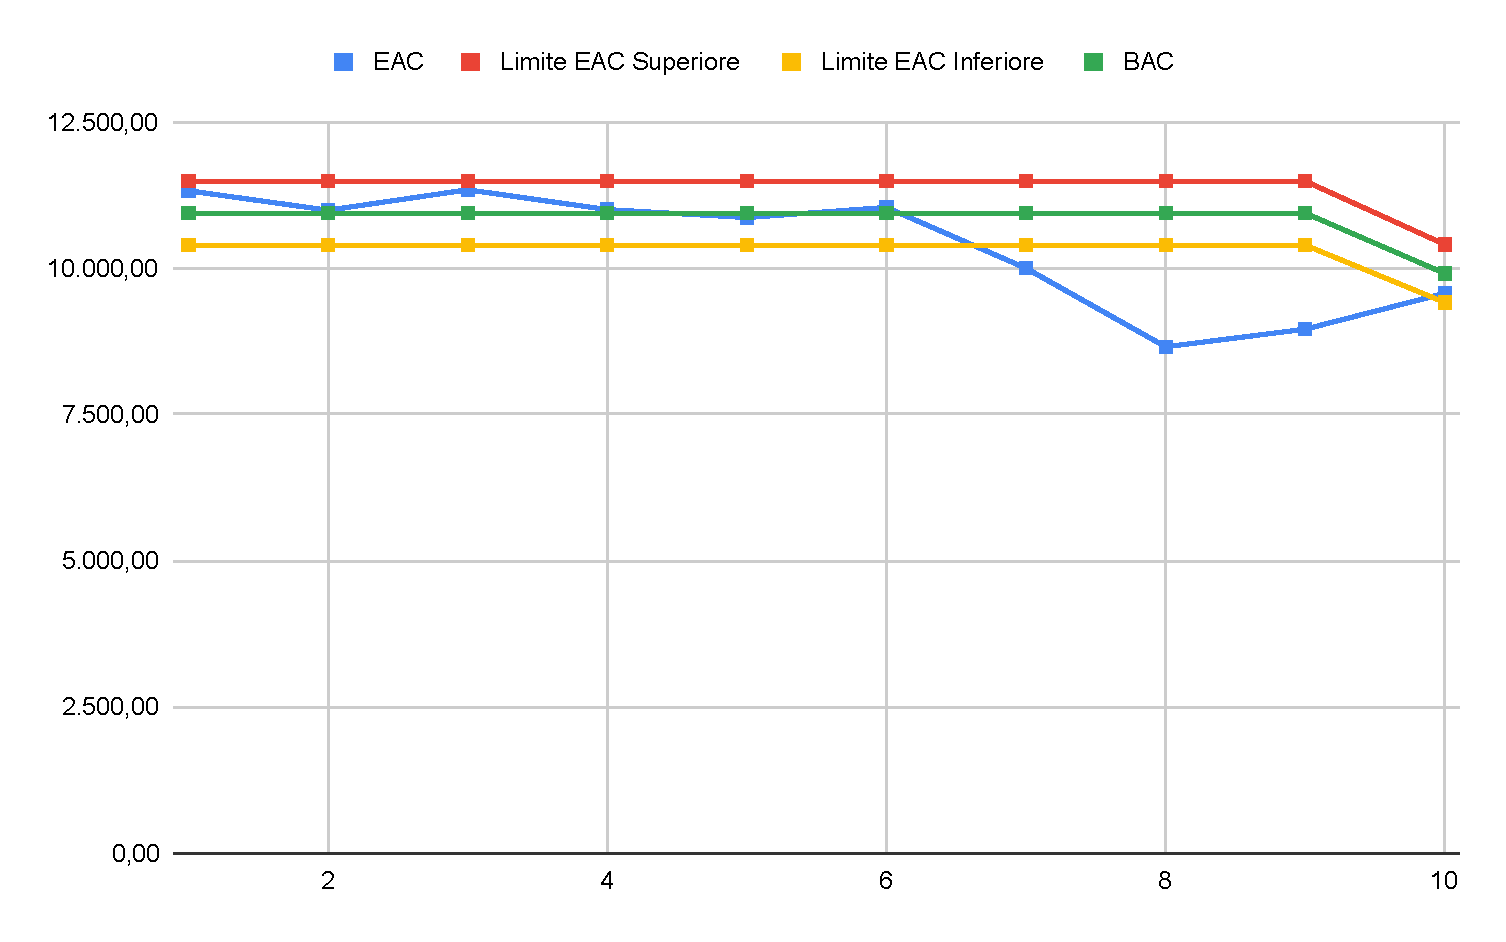
\includegraphics[width=0.9\linewidth]{resources/EAC.pdf}
    \caption{Estimated at Completion}
\end{figure}
Dal grafico si osserva l'andamento dell'EAC nei dodici sprint. Nel terzo periodo il valore si mantiene al di sopra del BAC, indicando una tendenza al superamento del budget pianificato; tuttavia, la traiettoria mostra un progressivo avvicinamento alla linea di base, suggerendo un miglioramento nella gestione delle risorse. Nel settimo e ottavo periodo invece si nota uno scostamento del valore EAC oltre il limite inferiore, dovuto ad un aumento dell'efficienza da parte del gruppo. Nel decimo periodo il gruppo ha riorganizzato la distribuzione delle ore, riducendo quelle inizialmente previste per ruoli di responsabile e analista a favore di amministratore e programmatore, pur rispettando i vincoli orari stabiliti. Questa riallocazione ha comportato una diminuzione del preventivo complessivo del progetto. Al termine del decimo sprint, il progetto risulta comunque rientrato nei limiti accettabili (±5\% BAC), condizione mantenuta anche nei periodi successivi.

\subsection{PC02-PV (Planned Value) e PC04-EV (Earned Value)}
\begin{figure}[H]
    \centering
    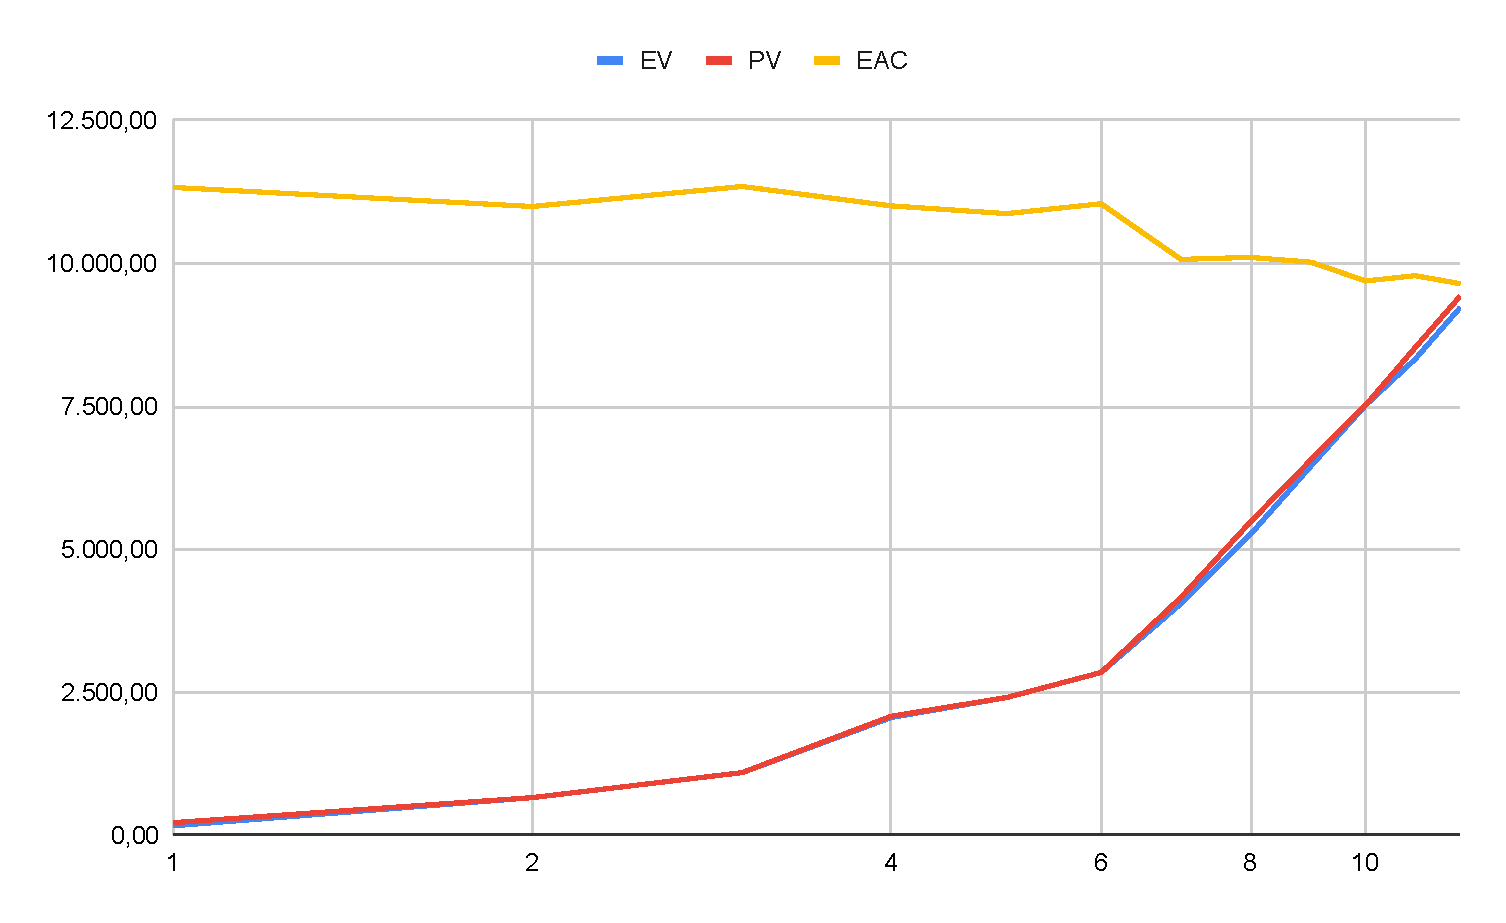
\includegraphics[width=0.9\linewidth]{resources/EV rispetto a PV.pdf}
    \caption{Planned Value - Earned Value}
\end{figure}
Il grafico mostra un andamento sostanzialmente allineato tra Planned Value (PV) ed Earned Value (EV) nel corso dei dodici sprint. Le due curve risultano quasi sovrapposte, a conferma che il gruppo sta producendo valore in linea con quanto pianificato. Questo indica una buona capacità di rispettare la pianificazione e di mantenere il ritmo di avanzamento previsto.

\subsection{PC05-ETC (Estimated to Complete)}
\begin{figure}[H]
    \centering
    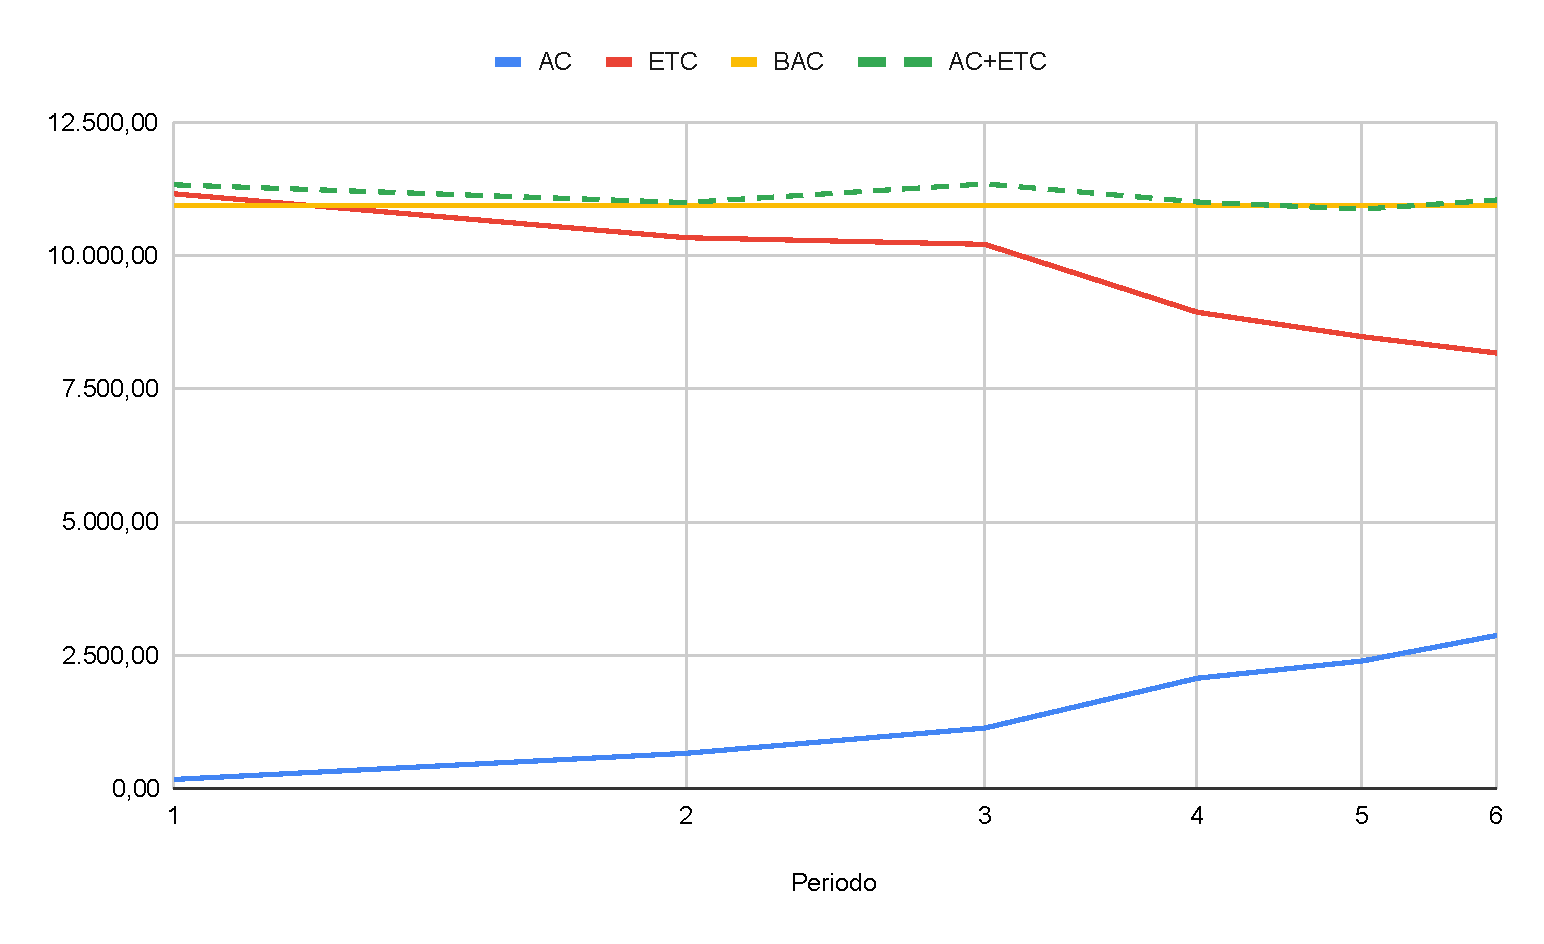
\includegraphics[width=0.9\linewidth]{resources/ETC.pdf}
    \caption{Estimated to Complete}
\end{figure}
Il grafico mette in relazione AC, ETC, BAC e la loro somma AC+ETC nel corso dei dodici sprint. La linea AC+ETC, che rappresenta la proiezione del costo finale, si mantiene al di sopra del BAC per i primi tre periodi, confermando un rischio di sforamento del budget stimabile intorno al 3--4\%. Tuttavia, nel quarto sprint si osserva un avvicinamento della linea AC+ETC al BAC, segnale positivo di un progressivo rientro nei costi pianificati. Dal quinto sprint in poi, la linea AC+ETC si mantiene prossima al valore desiderato (BAC). Dal settimo sprint inoltre si osserva una diminuzione della proiezione AC+ETC, risultato di un aumento della produttività del gruppo. È opportuno mantenere questo trend nei periodi conclusivi per minimizzare lo scarto finale.
Dal decimo sprint la linea AC+ETC, grazie alla redistribuzione delle ore si trova quasi nello stesso punto della linea del BAC.

\subsection{PC06-CV (Cost Variance), PC07-SV (Schedule Variance) e PC08-BV (Budget Variance)}
\begin{figure}[H]
    \centering
    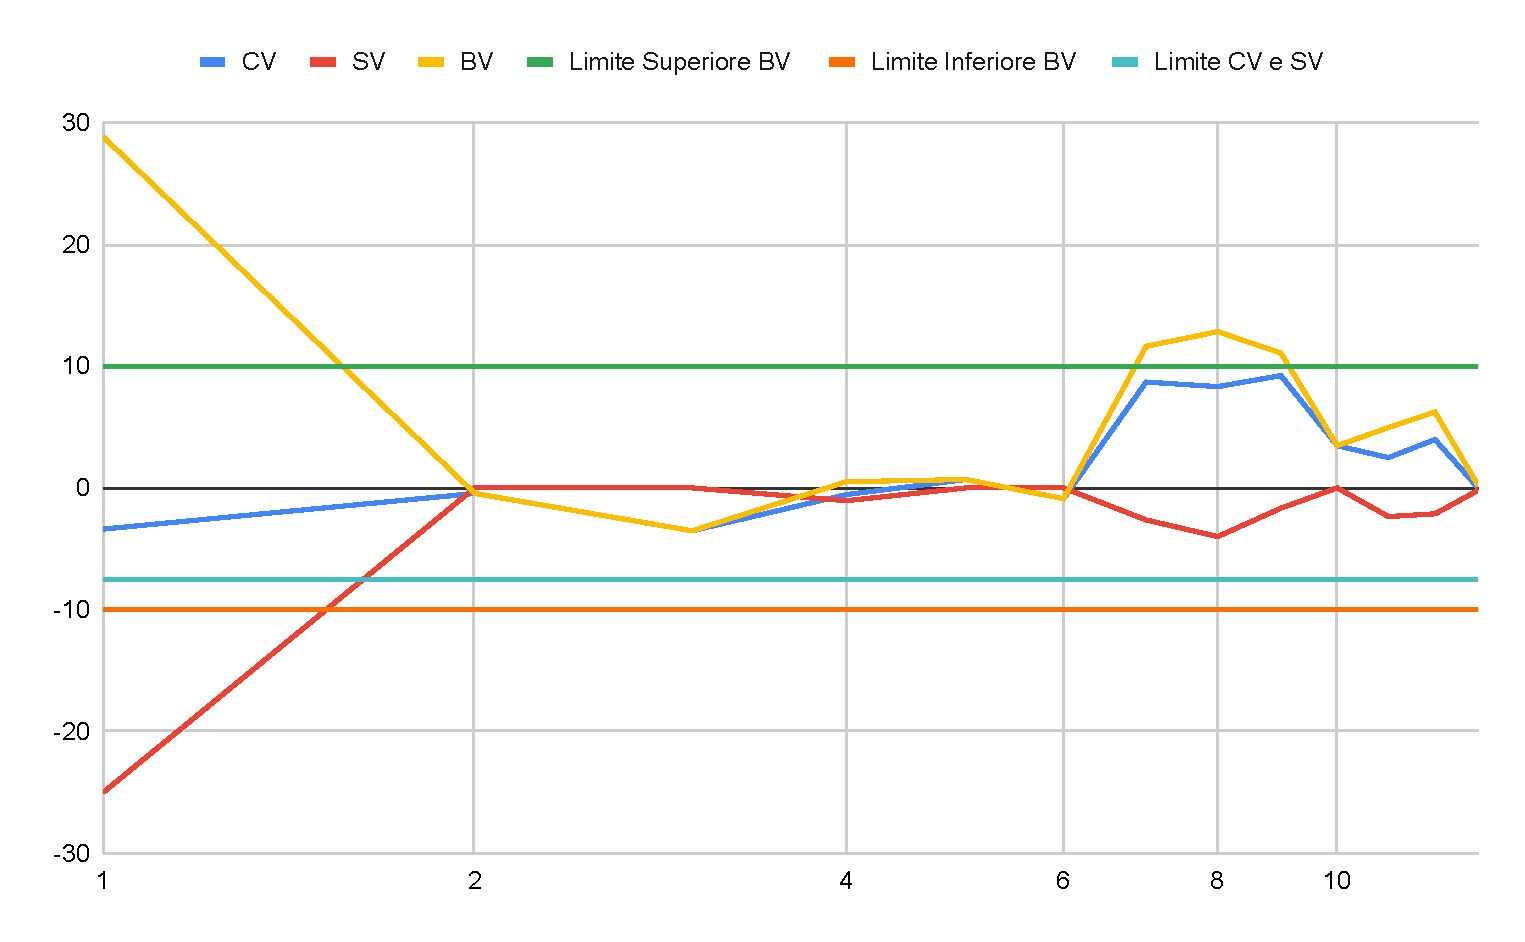
\includegraphics[width=0.9\linewidth]{resources/CV, SV, BV.pdf}
    \caption{Cost Variance, Schedule Variance e Budget Variance}
\end{figure}
Il grafico illustra l'andamento delle tre varianze nei dodici sprint$^G$: al termine del terzo sprint$^G$ si osserva un avvicinamento di CV e BV al limite inferiore, dovuto al periodo di sessione universitaria parzialmente previsto; la SV è rimasta stabile, suggerendo che il team ha deliberatamente pianificato meno lavoro in quel periodo per far fronte alla sessione, contenendo il ritardo sulla pianificazione a scapito però dell'efficienza$^G$ economica. Nel quarto sprint$^G$ CV e BV recuperano correttamente, tuttavia la SV mostra un leggero decremento, indicando che il rallentamento del terzo sprint$^G$ non è stato pienamente recuperato in termini di valore prodotto. Per il quinto e sesto sprint i valori si mantengono prossimi allo zero, evidenziando un recupero efficace e un riallineamento complessivo rispetto agli obiettivi pianificati. Nel settimo e ottavo sprint inoltre si nota un innalzamento di CV e BV dovuto ad un aumento della produttività del gruppo rispetto ai periodi precedenti. Dal decimo sprint, grazie alla ridistribuzione delle ore con conseguente ricalcolo del preventivo, viene registrato un reallineamento delle varianze entro i limiti accettabili.

\subsection{Indice di Gulpease}
\begin{figure}[H]
    \centering
    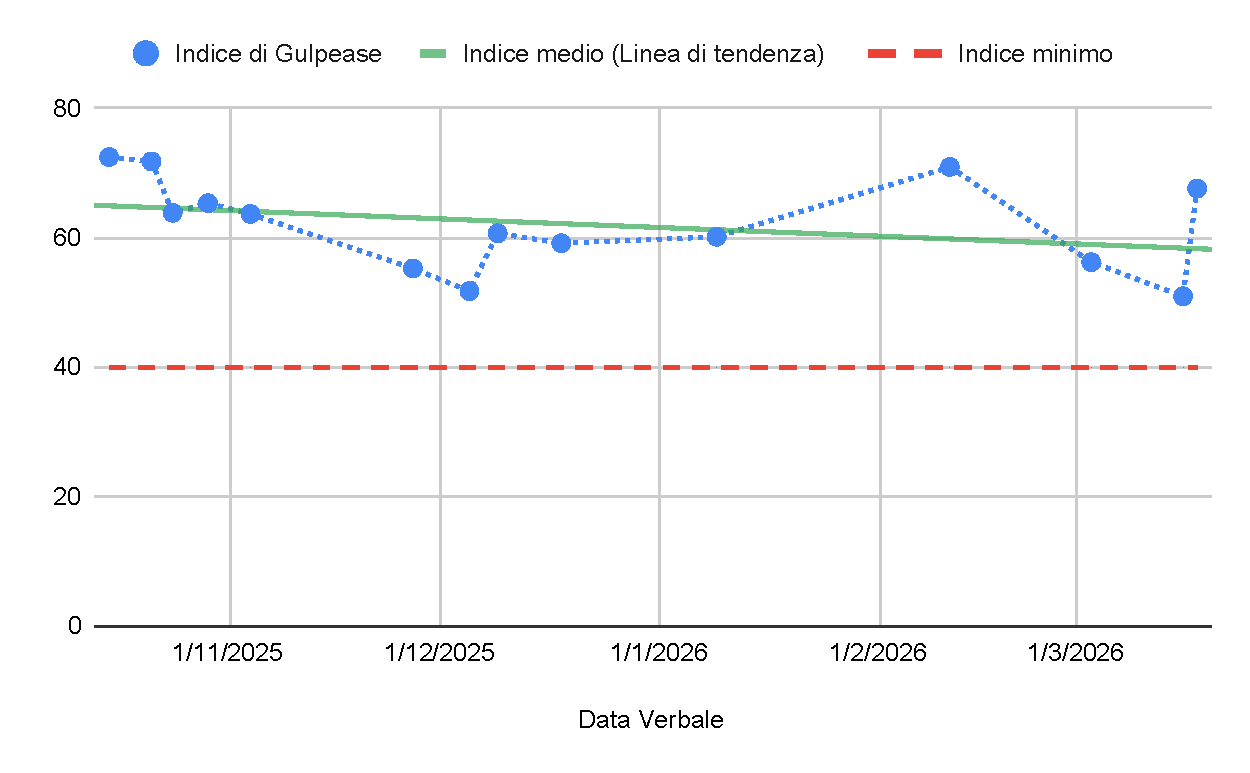
\includegraphics[width=0.9\linewidth]{resources/Andamento indice di Gulpease verbali.pdf}
    \caption{Andamento indice di Gulpease verbali}
\end{figure}
I risultati mostrano che tutti i verbali analizzati superano ampiamente la soglia minima accettabile di 40 punti nell'Indice di Gulpease, attestandosi su un valore medio di circa 60, a indicare una leggibilità complessivamente buona.

\begin{figure}[H]
    \centering
    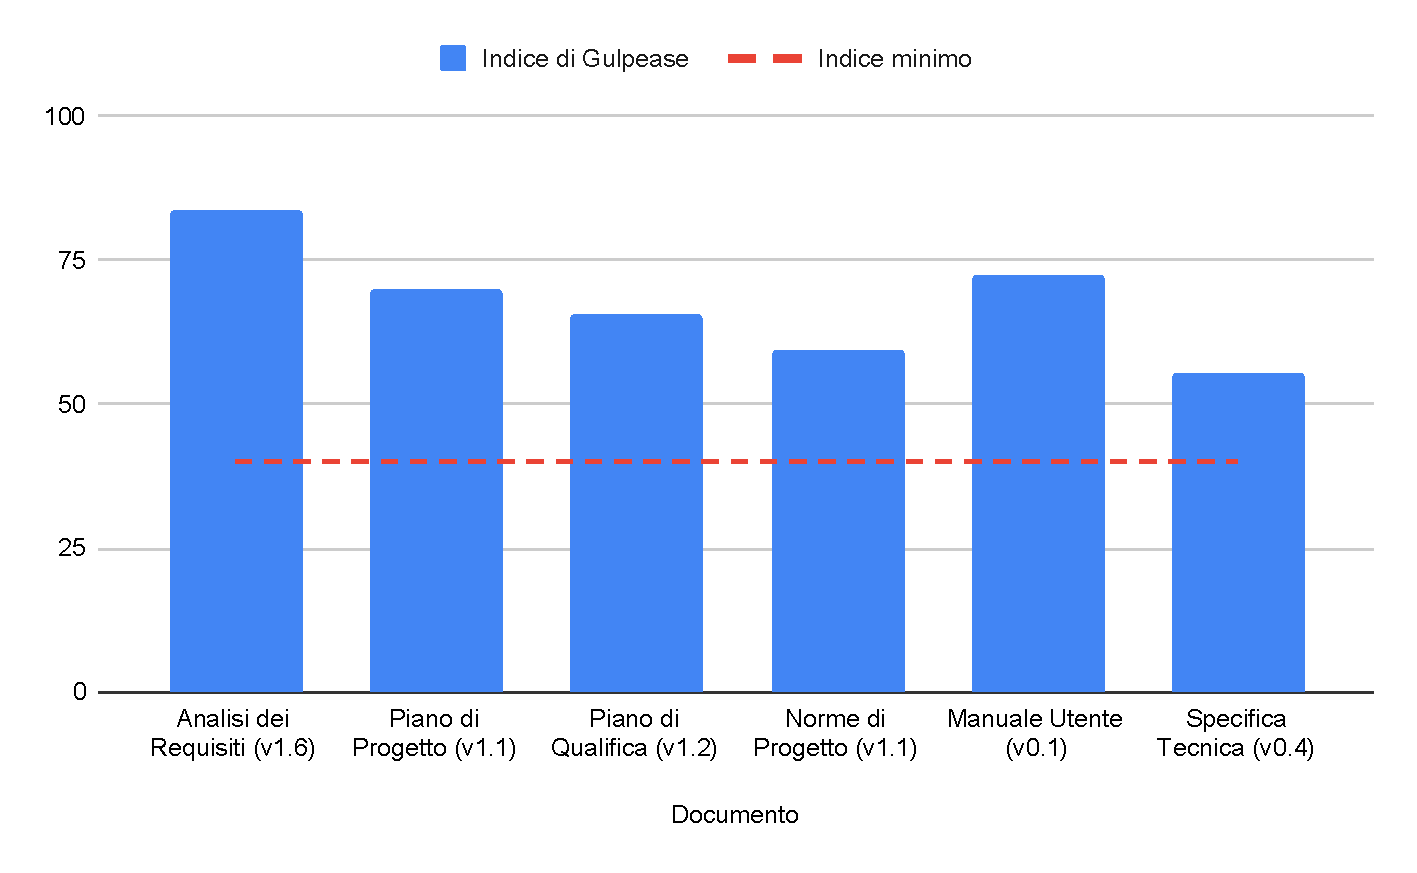
\includegraphics[width=0.9\linewidth]{resources/Indice di Gulpease documenti.pdf}
    \caption{Indice di Gulpease documenti RTB}
\end{figure}
Il grafico illustra i valori dell'Indice di Gulpease calcolati per i documenti Analisi dei Requisiti$^G$, Norme di Progetto$^G$, Piano di Progetto$^G$, Piano di Qualifica, Manuale Utente e Specifica Tecnica. Tutti i documenti superano abbondantemente la soglia minima di 40 punti. In particolare, l'Analisi dei Requisiti$^G$ registra un valore particolarmente elevato, riconducibile alla natura stessa del documento, caratterizzato da una struttura ricca di elementi grafici (Casi d'uso$^G$) e da un uso esteso di elenchi puntati, fattori che incidono positivamente sul calcolo dell'indice.

\subsection{PC15-PCTS (Percentuale dei test superati)}
Per quanto riguarda la percentuale dei test superati, dal momento della loro introduzione nel corso dell'undicesimo periodo, il loro superamento è sempre stato verificato prima dell'effettivo merge all'interno del branch develop. A parte dunque un primo periodo in cui non era ancora completata appieno l'automazione di \textit{test coverage} all'interno del repository, si è sempre ottenuto una percentuale di test superati pari al 100\%.
\begin{table}[H]
\centering
\renewcommand{\arraystretch}{1.2}
\begin{tabular}{|l|p{2.5cm}|p{2.5cm}|p{2.5cm}|p{2.5cm}|}
\hline
\textbf{Metrica} & \textbf{Nome} & \textbf{Valore Accettabile} & \textbf{Valore Preferibile} & \textbf{Valore ottenuto} \\
\hline
PC15-PCTS & Percentuale dei test superati & $\geq 80\%$ & 100\% & 100\% \\
\hline
\end{tabular}
\label{tab:res-verifica}
\end{table}

\subsection{PC16-SC (Statement Coverage)}
Lo Statement Coverage misura la percentuale di istruzioni eseguite durante l'esecuzione dei test. Si calcola come il numero di istruzioni eseguite almeno una volta rispetto al totale di istruzioni nel programma.
Il suo scopo è assicurarsi che tutte le istruzioni nel codice vengano testate almeno una volta. \\
Di seguito si riporta un immagine rappresentante la percentuale di Statement Coverage relativa a quelle che Codecov considera come \textit{"relevant lines"}, per ciascun file contenente codice coperto da test.
\begin{figure}[H]
    \centering
    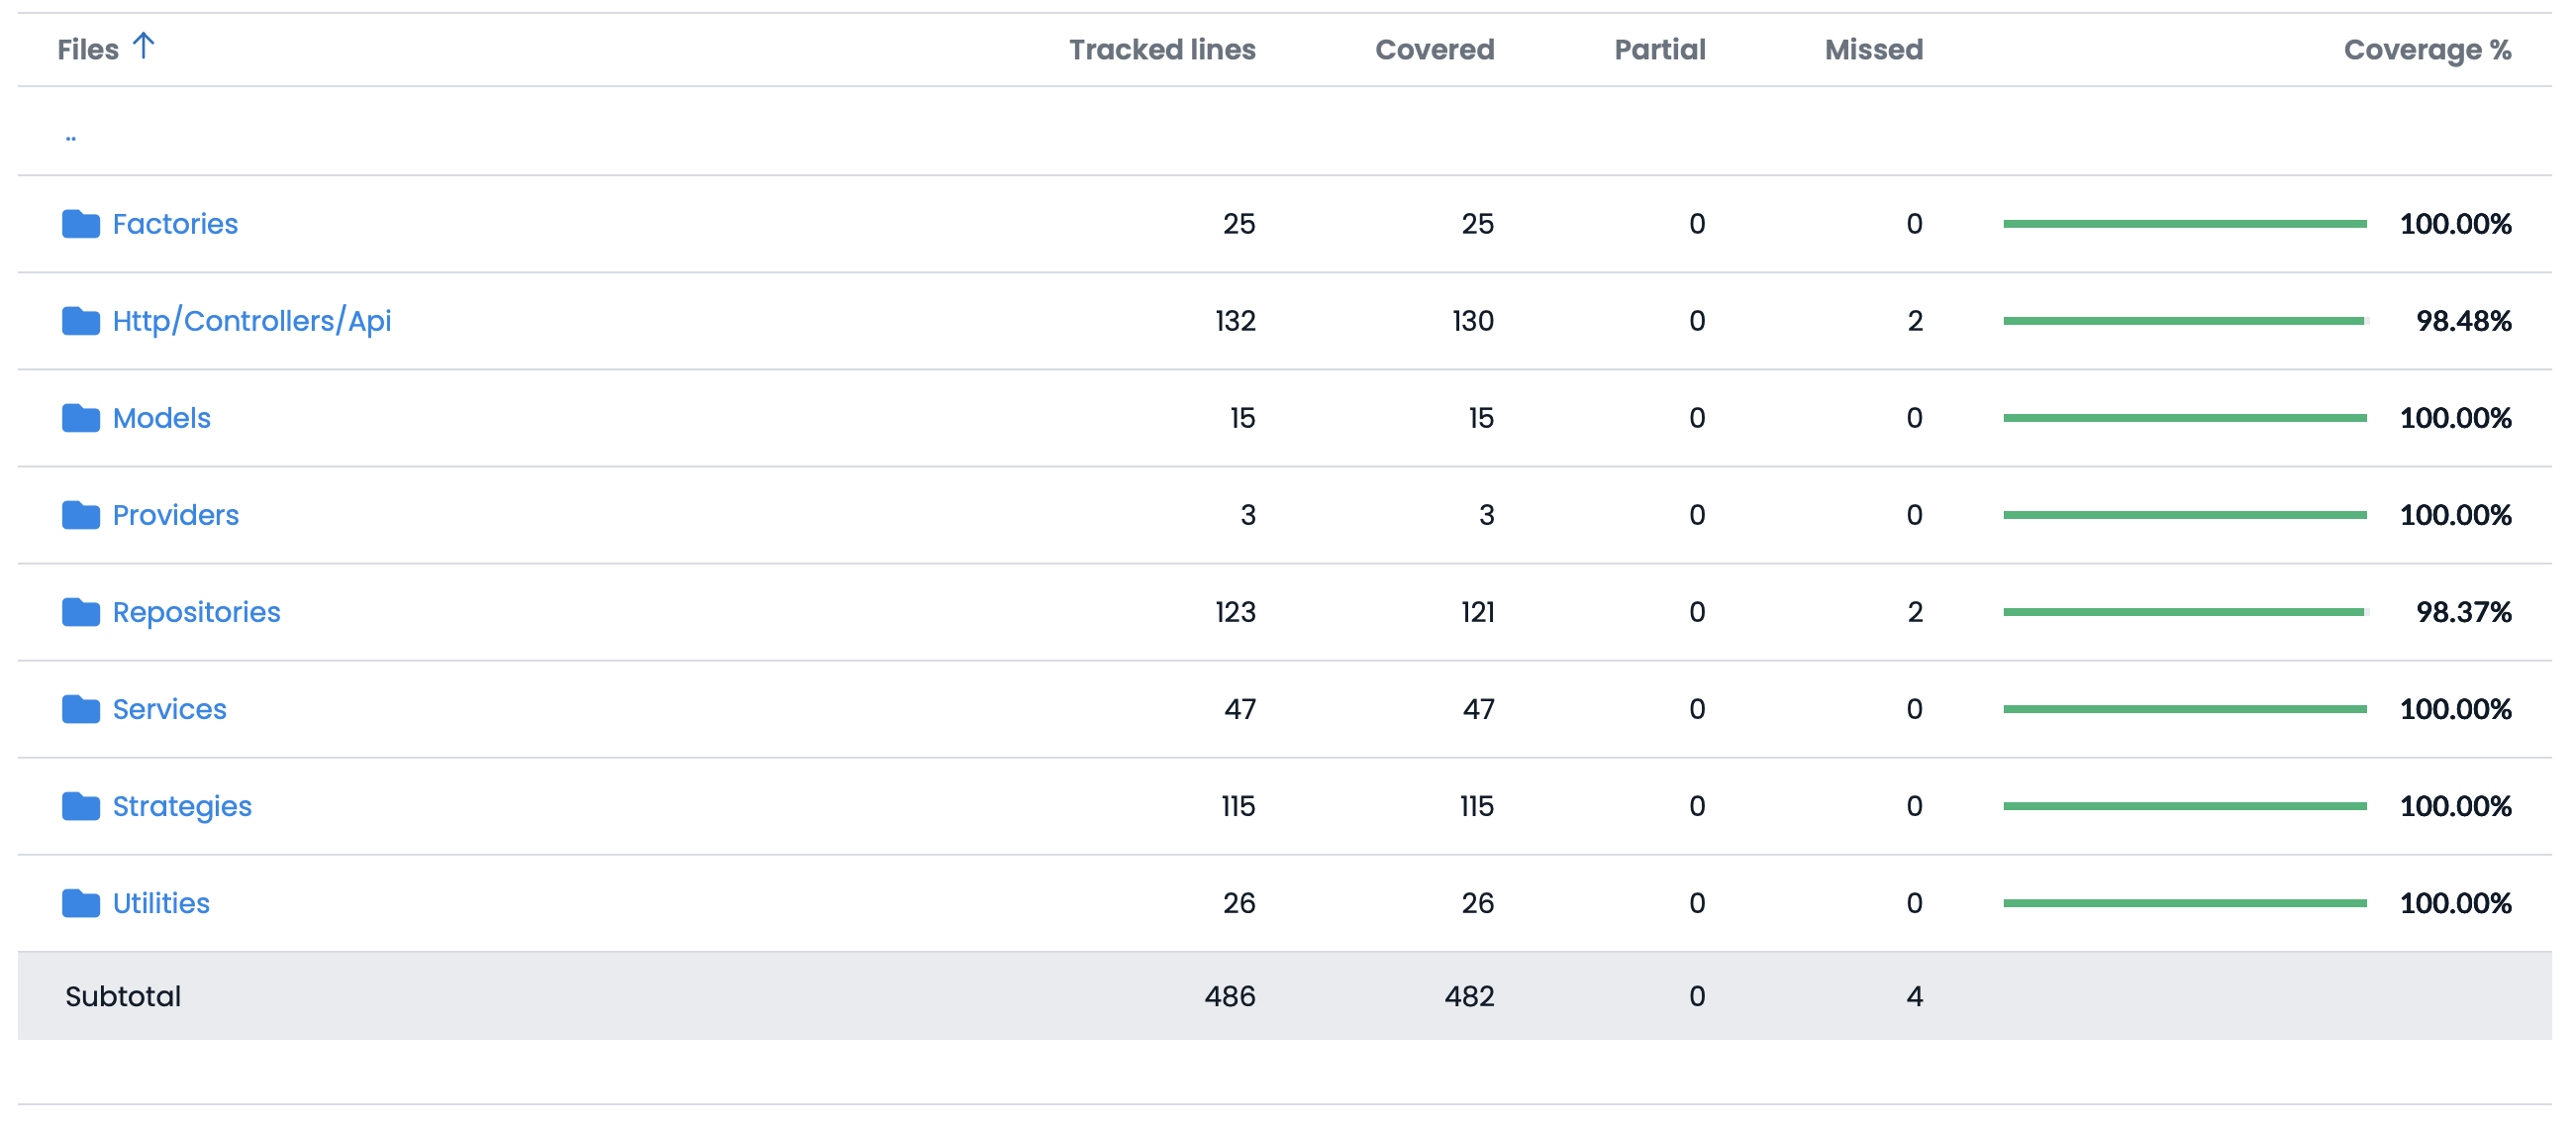
\includegraphics[width=0.9\linewidth]{resources/Statement Coverage.png}
    \caption{Statement Coverage}
\end{figure}

\section{Valutazioni per il miglioramento}
Questa sezione è dedicata alla valutazione generale del lavoro, con lo scopo di inserire osservazioni sui problemi riscontrati e sulle possibili correzioni da adottare.
\subsection{Valutazione sull'organizzazione}
\begin{table}[H]
\centering
\renewcommand{\arraystretch}{1.2}
\begin{tabular}{|p{3cm}|p{4cm}|p{2cm}|p{4cm}|}
\hline
\textbf{Problema} & \textbf{Descrizione} & \textbf{Gravità} & \textbf{Soluzione} \\
\hline
Tracciamento temporale &
Inizialmente è stato difficile tracciare le ore per ogni attività del ruolo coperto da ogni membro &
Media &
Utilizzo di issue su GitHub per suddividere ogni attività in base allo sprint, con relativo tracciamento temporale \\
\hline
\end{tabular}
\caption{Valutazione sull’organizzazione}
\label{tab:valutazione-organizzazione}
\end{table}

\subsection{Valutazione degli strumenti utilizzati}
\begin{table}[H]
\centering
\renewcommand{\arraystretch}{1.2}
\begin{tabular}{|p{3cm}|p{4cm}|p{2cm}|p{4cm}|}
\hline
\textbf{Problema} & \textbf{Descrizione} & \textbf{Gravità} & \textbf{Soluzione} \\
\hline
Suddivisione task &
Il gruppo ha spesso riscontrato problemi sulla divisione di task &
Bassa &
Creazione di sub-issue in modo da assegnare allo specifico membro la sua parte di issue da eseguire \\
\hline
\end{tabular}
\caption{Valutazione degli strumenti utilizzati}
\label{tab:valutazione-strmenti}
\end{table}

\subsection{Valutazione sui ruoli}
\begin{table}[H]
\centering
\renewcommand{\arraystretch}{1.2}
\begin{tabular}{|p{3cm}|p{4cm}|p{2cm}|p{4cm}|}
\hline
\textbf{Problema} & \textbf{Descrizione} & \textbf{Gravità} & \textbf{Soluzione} \\
\hline
Responsabile &
La partizione dei compiti e la gestione delle ore, prima dell'utilizzo delle issue su GitHub, era vaga e poco accurata &
Media &
Grazie alle issue su GitHub è possibile possibile tenere traccia delle ore impiegatate per ciascun task e quindi fare il resoconto dei costi e dei tempi rispetto al preventivo \\
\hline
\end{tabular}
\caption{Valutazione sui ruoli}
\label{tab:valutazione-ruoli}
\end{table}

\end{document}
